% This is LLNCS.DEM the demonstration file of
% the LaTeX macro package from Springer-Verlag
% for Lecture Notes in Computer Science,
% version 2.4 for LaTeX2e as of 16. April 2010
%
\documentclass[10pt, journal, twocolumn, final, a4paper]{IEEEtran}
%
\usepackage{makeidx}  % allows for indexgeneration
%

% allow for compress references ranges (IEEEtran_HOWTO S.VII)
% noadjust removes a leading space before the []
\usepackage[noadjust]{cite}


\usepackage[english,activeacute]{babel}
\usepackage[english]{layout}
\usepackage{amsfonts,amssymb}
\usepackage[cmex10]{amsmath}
\usepackage{amsopn} % DeclareMathOperator
\usepackage{amsbsy} % boldsymbol
\usepackage[dvips]{graphicx}
\usepackage{color}
\usepackage{subfig}
\usepackage{colonequals}
\usepackage[latin1]{inputenc}
\usepackage{url}
\usepackage{epsfig}
\usepackage{dsfont}
\usepackage{multirow}

\usepackage{algorithm}
\usepackage{algorithmic}
\usepackage{setspace}
\usepackage{afterpage}
%\usepackage{showkeys}
% \usepackage{mathptmx}      % use Times fonts if available on your TeX system
% \usepackage{latexsym}

%\usepackage[left=1.2in,right=1.2in]{geometry}

% \graphicspath{{../iccv09/}}

%\newcommand{\best}[1]{\textbf{\textcolor{MyOrange}{#1}}}
\newcommand{\best}[1]{#1}
\newcommand{\bsic}[1]{\textcolor{black}{\textit{#1}}}
\newcommand{\Bsic}[1]{\textcolor{black}{\textbf{\textit{#1}}}}
\newcommand{\Best}[1]{\textbf{\textcolor{black}{#1}}}

\newcommand{\ma}[1]{\boldsymbol{#1}}
\newcommand{\tras}[1]{#1^{\mathrm{T}}}
\newcommand{\herm}[1]{#1^{\mathrm{H}}}
\newcommand{\con}[1]{#1^{\mathrm{*}}}
\newcommand{\E}{\mathds{E}}
\newcommand{\tech}[1]{\overline{#1}}
\newcommand{\nspace}{\!\!\!\!}
\newcommand{\nmbr}[1]{\oldstylenums{#1}}

\newcommand{\eg}{\emph{e.g}. } \newcommand{\Eg}{\emph{E.g}. }
\newcommand{\ie}{\emph{i.e}. } \newcommand{\Ie}{\emph{I.e}. }
\newcommand{\cf}{\emph{c.f}. } \newcommand{\Cf}{\emph{C.f}. }
\newcommand{\etc}{\emph{etc}. } \newcommand{\vs}{\emph{vs}. }
\newcommand{\wrt}{w.r.t\onedot } \newcommand{\dof}{d.o.f. }
\newcommand{\etal}{\emph{et al}. }

\newcommand{\R}{\mathds{R}}
\newcommand{\sign}{\mathrm{sign}}
\newcommand{\eps}{\varepsilon}
\newcommand{\To}{\longrightarrow}
% \newcommand{\II}{1{\hskip -2.5 pt}\hbox{I}}

\renewcommand{\algorithmiccomment}[1]{\bgroup\hfill\small\textcolor{gray}{//~#1}\egroup}

% c++ code
\usepackage{listings}
\usepackage{xcolor}
\usepackage{textcomp}
\definecolor{listinggray}{gray}{0.9}
\definecolor{lbcolor}{rgb}{0.9,0.9,0.9}
\lstset{
	backgroundcolor=\color{lbcolor},
	tabsize=4,    
%  rulecolor=,
	language=Matlab,
	basicstyle=\scriptsize\ttfamily,
	upquote=true,
	aboveskip={1.5\baselineskip},
	columns=fixed,
	showstringspaces=false,
	extendedchars=false,
	breaklines=true,
	prebreak = \raisebox{0ex}[0ex][0ex]{\ensuremath{\hookleftarrow}},
	frame=single,
	numbers=left,
	showtabs=false,
	showspaces=false,
	showstringspaces=false,
	identifierstyle=\ttfamily,
	keywordstyle=\color[rgb]{0,0,1}\ttfamily,
	commentstyle=\color[rgb]{0,0.5,0}\ttfamily,
	stringstyle=\color[rgb]{0.627,0.126,0.941}\ttfamily,
	numberstyle=\color[rgb]{0.5, 0.5, 0.5}\ttfamily,
%  \lstdefinestyle{C++}{language=C++,style=numbers}’.
}
%\lstset{
%	backgroundcolor=\color{lbcolor},
%	tabsize=4,
%	language=C++,
%	captionpos=b,
%	tabsize=3,
%	frame=lines,
%	numbers=left,
%	numberstyle=\tiny,
%	numbersep=5pt,
%	breaklines=true,
%	showstringspaces=false,
%	basicstyle=\footnotesize,
%	identifierstyle=\color{magenta},
%	keywordstyle=\color[rgb]{0,0,1},
%	commentstyle=\color{green},
%	stringstyle=\color{red}
%}
	
	
	


\DeclareMathOperator*{\argmin}{arg\,min}
\DeclareMathOperator*{\argmax}{arg\,max}

\newcommand{\nota}[1]{\textcolor{blue}{\textbf{#1}}}
\newcommand{\suggest}[1]{\textcolor{cyan}{#1}}
\newcommand{\add}[1]{\textcolor{green}{#1}}
\newcommand{\remove}[1]{\textcolor{red}{#1}}
\newcommand{\todo}[1]{\textcolor{red}{\noindent\textsc{todo}: #1}}
\newcommand{\dosdv}[1] {#1}
\newcommand{\uncite}[1] {}
% \newcommand{\tachar}[1]{
% \setbox4=\hbox{\ } \setbox3=\hbox{#1} \hbox{#1} \kern -\wd3 \kern
% -\wd4 \raise 0.3\ht3 \hbox{ \vrule width \wd3 height 0.5pt} }

% \theoremstyle{plain}\newtheorem{theorem}{Theorem}[chapter]
% \theoremstyle{plain}\newtheorem{proposition}{Proposition}[chapter]
% \theoremstyle{plain}\newtheorem{lemma}{Lemma}[chapter]
% \theoremstyle{definition}\newtheorem{definition}{Definition}[chapter]

% New definition of square root:
% it renames \sqrt as \oldsqrt
\let\oldsqrt\sqrt
% it defines the new \sqrt in terms of the old one
\def\sqrt{\mathpalette\DHLhksqrt}
\def\DHLhksqrt#1#2{%
\setbox0=\hbox{$#1\oldsqrt{#2\,}$}\dimen0=\ht0
\advance\dimen0-0.2\ht0
\setbox2=\hbox{\vrule height\ht0 depth -\dimen0}%
{\box0\lower0.4pt\box2}}


\begin{document}

\title{A Non-local Bayesian Video Denoising Method}

\author{Pablo~Arias, Jean-Michel~Morel%
\thanks{P. Arias (\texttt{pablo.arias@upf.edu}) and J.-M. Morel
(\texttt{jean-michel.morel@cmla.ens-cachan.fr}) are with the \emph{Centre de
math\'ematiques et de leurs applications} (CMLA), \'Ecole Normale Sup\'eriore
de Cachan, 61 Av. du Pr\'esident Wilson, F-94230 Cachan, France}}

\markboth{IEEE Transactions of Image Processing,~Vol.~X, No.~X, Month~2015}%
{Arias, Morel: A Non-local Bayesian Video Denoising Method}


\maketitle              % typeset the title of the contribution

\begin{abstract}
	The quality provided by image/video sensors increases steadily, and
	for a fixed spatial resolution the sensor noise has been gradually reduced.
	However, modern sensors are also capable of acquiring at higher spatial
	resolutions which are still affected by noise, specially at low lighting
	conditions. The situation is even worse in video cameras, where the capture
	time is bounded by the frame rate. The noise in the video degrades its visual 
	quality and hinders its analysis.
	In this paper we present a new video denoising method extending 
	the non-local Bayes image denoising algorithm. The method does not require 
	motion estimation, and yet preliminary results show that it outperforms the
	state-of-the-art methods in terms of PSNR.
\end{abstract}

% Note that keywords are not normally used for peerreview papers.
\begin{IEEEkeywords}
	video denoising, Bayesian methods, patch-based methods
\end{IEEEkeywords}


% For peer review papers, you can put extra information on the cover
% page as needed:
% \ifCLASSOPTIONpeerreview
% \begin{center} \bfseries EDICS Category: 3-BBND \end{center}
% \fi
%
% For peerreview papers, this IEEEtran command inserts a page break and
% creates the second title. It will be ignored for other modes.
\IEEEpeerreviewmaketitle

%
\section{Introduction}
%

Advances in video sensor hardware have steadily improved the acquisition
quality. However, due to the reduction in the price of cameras
and data storage, video cameras are being used more each time, and in less
favorable situations, such as low lighting conditions. This results in high 
levels of noise, which negatively affects the visual quality of the video and
hinders its use for any application. 
\todo{Add references for claims about sensors, camera prices, etc.}

Video denoising has received much less attention than still image denoising. 
In principle, video denoising should be easier than image denoising, since the
strong temporal redundancy along motion trajectories favours the denoising
task. However, this additional form of redundancy creates challenges.  On one
hand, the amount of data is much larger than for still images, and efficient
ways of navigating through this data are needed. On the other hand, the output
of the denoising algorithm should be temporally consistent according to the
motion of the original sequence.

Early works proposed temporal or spatio-temporal filters which either compensate
for motion on estimated motion trajectories or used some kind of mechanism to
adapt to the changes in the video signal at a fixed location due to the motion.
We refer the reader to \cite{Brailean1995a} and references therein for more details.
Other video denoising works apply temporal filtering to the wavelet coefficients 
of the frames \cite{Jin2006,Zlokolica2006a}. 

Some methods do not distinguish between the temporal and spatial dimensions,
and treat the video as a volume, which is denoised in a transformed domain
\cite{Rajpoot2003,Wilson2004,Selesnick2003}. 
\todo{Read these references. Even if they consider a 3D transform, I think
they DO distinguish between space and time}

Until the advent of patch-based approaches, methods that do not compensate
motion failed for sequences with moderate motion, and their main interest resided
in their simplicity and low computational cost. First state-of-the-art results
obtained without motion estimation were reported in \cite{Buades2005v}, with the
non-local means algorithm. The authors argued that for their method, based on
averaging similar patches, motion estimation was not only unnecessary but
counterproductive: while textured regions are problematic for motion
estimation, they are a source of a large number of similar patches across
different frames. Even if the motion trajectory could be reliably estimated, it
makes more sense to use all similar patches, rather than using only the ones on the
trajectory.
%
A similar approach was followed by the authors of \cite{Dabov2007v}. This method is based
on collaborative filtering of similar patches in a
spatio-temporal neighborhood. 

The methods in \cite{Buades2005v} and \cite{Dabov2007v} are extensions to video
of still image patch-based denoising algorithms (non-local means REF and BM3D
REF respectively). They are based on \suggest{filtering} similar 2D patches
searched for in a 3D spatio-temporal neighborhood.  These methods exploit both
spatial and temporal redundancy, however, since each 2D patch is processed
independently, there is no mechanism to impose coherence along trajectories.
This results in flickering artifacts which become noticeable for high levels of
noise. 
%
While these methods exploit spatio-temporal redundancy, they do not impose
coherence of the trajectories, resulting in flickering
artifacts which become noticeable for high levels of noise. 

A natural next step is to consider 3D spatio-temporal patches. This has two
main advantages (at the expense of a higher computational cost). First it
provides a mechanism to impose some temporal consistency on the result, since
now, the temporally continguous 2D spatial slices of a spatio-temporal patch
are filtered jointly. Secondly, a 3D patch has a higher number of pixels
resulting in a reduction of the noise in the distance between patches. On the
other hand, to get the same reduction in the distance noise with 2D patches one
needs to increase their spatial size which leads to a smaller number of similar
patches.

Two types of 3D patches have been used: rectangular and motion-compensated.
Motion-compensated 3D patches follow a motion trajectory previously estimated.
Each approach has its pros and cons.

Motion-compensated patches have the benefit that their spatial slices are very
similar between each other (or the same, assuming purely translational pixelic
motion). As a consequence, temporal filtering can be easily performed by
filtering inside the patch in the temporal direction. 
Because of this, methods that use motion-compensated 3D patches only look for
similar motion-compensated 3D patches starting in the same frame.


%It has been shown by \cite{Liu2010} and \cite{Maggioni2011,Maggioni2012} that motion estimation can still be
%beneficial for patch-based methods. 
%
An example of this is the method presented in \cite{Liu2010}. The authors
propose a method based on non-local means. The method is described in terms of
2D patches. To denoise a target 2D patch, the $k$ nearest neighbors in the current
frame are found. The 2D patches in their forward and backward trajectories are
used also to denoising the target patch. As a consequence the set of similar
patches averaged to denoise each pixel varies smoothly along motion
trajectories. This yields results with high temporal consistency. 
To estimate motion, their method resorts to a robust optical flow algorithm
based on \cite{Bruhn2005}.

In \cite{Maggioni2011,Maggioni2012}, the authors introduced V-BM4D, an
extension of BM3D to video by collaborative filtering of similar motion
compensated 3D patches. Trajectories are computed with a block matching
strategy based on the sum of squared differences (SSD) and a temporal
regularization term, which favours trajectories with small velocity and low
acceleration. The results of this algorithm show higher PSNR and temporal
consistency, resulting in a higher overall quality.

One of the main difficulties in using motion-compensated patches is estimating
motion. Motion estimation is a paramount problem in noiseless sequences, and
noise makes it much harder.

Rectangular 3D patches offer an appealing
alternative, since they do not require estimating motion. 
In \cite{Protter2007,Protter2009} the authors extend the K-SVD \cite{Elad2006}
image denoising method to video by learning a dictionary of spatio-temporal
rectangular 3D patches.

Each rectangular 3D patch results from the combination of a 2D texture and a
motion pattern. For arbitrary motion, each combination of texture and motion is
not likely to occur together again. Thus rectangular 3D patches should have
less repeatability in the video compared to motion compensated patches.  An
exception is when the motion is a global translation of the frame, in which
case, the motion pattern is equal for each patch. Furthermore, if there is no
acceleration (uniform motion), rectangular 3D patches are constant along motion
trajectories. Global uniform motion is indeed a too restrictive model, but in
many cases, it is a valid approximation in a local neighborhood in space and
time.

\bigskip

In this work we present an extension to video of the non-local Bayes image
denoising method \cite{Lebrun2013a,Lebrun2013ipol} using 3D rectangular
patches and which does not require motion estimation. Yet, it provides
results which compare favourably to the current state-of-the-art,
both quantitatively by a significant marging and qualitatively, specifically in
terms of the temporal consistency attained.

\bigskip

The rest of the paper is structured as follows: in \S
\ref{sec:review_nonlocal_Bayes} we review the Bayesian patch denoising principle 
and describe our extension to video. In \S \ref{sec:parameters}
we discuss its parameters. Some results, including a comparison with VBM4D, are shown
in \S \ref{sec:results}. Concluding remarks are given in \S \ref{sec:conclusion}

\section{Bayesian video denoising}
\label{sec:review_nonlocal_Bayes}

A patch based Bayesian algorithm can assume that the patches similar to a given
patch follow a Gaussian distribution.
The problem 
of denoising can then be formulated as a problem of optimal Bayesian inference, where the
parameters of the prior are learnt from the noisy data.

\subsection{A nonlocal Bayesian principle}

Consider a grayscale video $u:\Omega\times \{1,\cdots,T\}\rightarrow
\mathbb R$, where $\Omega$ is the spatial domain (a rectangular discrete grid).
We assume that $v$ is a noisy version of $u$, contaminated with additive,
Gaussian, white noise $n$ of known variance $\sigma^2$,
\[v = u + n.\]

Given a rectangular 3D patch $\ma q$ of size $s_x\times s_x\times s_t$ of the noisy video $v$, and the 
corresponding patch $\ma p$ of the clean video $u$, we assume the following 
Gaussian linear model of $\ma p$ and $\ma q$:
\begin{align}
	\mathds{P}(\ma p) &= \mathcal N(\overline {\ma p}, C) \propto \exp\left(-\frac12\langle \ma p - \overline{\ma p}, C^{-1}(\ma p - \overline{\ma p})\rangle\right) \label{eq:prior}\\
	\mathds{P}(\ma q|\ma p) &= \mathcal N(\ma p, \sigma I) \propto \exp\left(-\frac1{2\sigma^2}\|\ma q - \ma p\|^2\right) \label{eq:obs}
\end{align}
Once the mean patch $\overline{\ma p}$ and the
covariance matrix $C$ have been estimated from the image itself, the MAP
estimate $\widetilde{\ma p}$ given a noisy patch $\ma q$ is obtained as:
\[ \widetilde{\ma p} = \argmax_{\ma p} \mathds P(\ma p | \ma q) = \argmin_{\ma p} -\log \mathds P(\ma p | \ma q). \]
Since we are working with Gaussian distributions, the log-posterior is a quadratic (positive definite)
function and the MAP can be computed explicitly as (see  \cite{Lebrun2013a})
\begin{equation}
	\widetilde{\ma p} = \overline{\ma p} + C(C + \sigma^2 I)^{-1}(\ma q - \overline{\ma p})
	\label{eq:map}
\end{equation}
The matrix in the above equation can be diagonalized in the basis of
principal directions of the covariance matrix $C$.
Let $C = U\Lambda U^T$ denote the eigendecomposition of $C$. Then we have that
\[U^T(\widetilde{\ma p} - \overline{\ma p}) \,\,\,\, = \,\,\,\, 
	\Lambda(\Lambda + \sigma^2 I)^{-1}\,\,\,\,
	U^T (\ma q - \overline{\ma p}).\]
The diagonal operator $W = \Lambda(\Lambda + \sigma^2I)^{-1}$
has the following coefficients:
\begin{equation}
w_{ii} = \frac{\lambda_i}{\lambda_i + \sigma^2}
	%	       = (1 + \sigma^2/\lambda_i)^{-1}
				 = (1 + \text{snr}_i^{-1})^{-1}
				 \label{eq:wiener_coeffs}
\end{equation}
which correspond to a Wiener filter on the principal components.

%
%In practice, we introduce a parameter $\beta$ (with $\beta \approx 1$)
%multiplying $\sigma^2I$ to be able to control the amount of filtering.

\subsection{Learning a low-rank \textit{a priori} model}

The parameters of the \textit{a priori} model, are learnt from the noisy video as
follows. For each noisy patch $\ma q$, we select the most $N_{\text{sim}}$
similar 3D patches found in a search region centered at $\ma q$. The
search region is a spatio-temporal rectangle of size $n_x \times
n_x \times n_t$ ($n_x, n_t$ are odd numbers). 

Let us note by $\ma q_i$, $i = 1, \dots, N_{\text{sim}}$ the set of patches
similar to $\ma q$ (with $\ma q_1 = \ma q$). We assume that these 
patches correspond to different noisy observations of the Gaussian linear model
\eqref{eq:prior} and \eqref{eq:obs}. The corresponding marginal distribution is given by
\[\mathds P(\ma q) = \mathcal N(\overline{\ma p}, C + \sigma^2I). \]
Therefore, the maximum likelihood estimates for $\overline{\ma p}$ and $C$ are given by 
\begin{equation}
	\widehat{\overline{\ma p}} = \frac1{N_{\text{sim}}}\sum_{i = 1}^{N_{\text{sim}}}\ma q_i \quad\text{and}\quad 
		\widehat C= \frac1{N_\text{sim}}\sum_{i = 1}^{N_{\text{sim}}}\ma q_i\ma q_i^T - \sigma^2I.
	\label{eq:learn_parameters}
\end{equation}

We will also assume that the covariance matrix has a lower rank $k$.  In this
case, it has been shown REF PPCA that maximum likelihood estimate is given by
truncated the spectral decomposition of $\widehat C$ to the $k$ largest
eigenvalues.
\begin{equation}
\widehat C_k = \sum_{i = 1}^k\widehat \lambda_i\widehat U_i\widehat U_i^T,
\end{equation}
where $\widehat \lambda_i$, $\widehat U_i$ denote the $i$-th largest
eigenvalue and its corresponding eigenvector respectively.

\bigskip

Other methods for image denoising have been proposed in the
literature based on Gaussian models for the patch density. In \cite{Yu2012},
the authors introduce a framework for solving inverse problems, based on the
assumption that the patches of an image are distributed according to a Gaussian
Mixture Model (GMM). A method is proposed to learn the parameters of the model from
the image. A GMM is also used in \cite{Zoran2011}, but it is trained from a
database of $2\cdot 10^6$ patches randomly sampled from the Berkeley database.

In \cite{Zhang2010} a PCA-based algorithm is introduced which is equivalent to 
the nonlocal Bayes method. In fact, nonlocal Bayes can be regarded as a Bayesian 
interpretation of \cite{Zhang2010}.

The BLS-GSM method \cite{Portilla2003} (Bayes least square estimate of Gaussian
scale mixture) models noiseless ``wavelet coefficient neighborhoods'' with a
Gaussian scale mixture defined as a random scaling of a zero-mean Gaussian
density. The wavelet coefficient neighborhood turns out to be a patch of an
oriented channel of the image at a given scale.



\section{Description of the algorithm}

Let us now describe the video denoising algorithm. As in
\cite{Dabov2007tip,Dabov2007v,Maggioni2012,Lebrun2013a} we perform two stages, described in 
Algorithms \ref{alg:nlbayes} and \ref{alg:nlbayes2}. In the first stage we
compute a \emph{basic} estimate, which we denote $\widetilde u^{(1)}$. 

In the second stage computes the final estimate $\widetilde u^{(2)}$ using the
basic estimate as an oracle. This entails two modifications with respect to the
first stage (highlighted in italics in Algorithm \ref{alg:nlbayes2}). Firstly, the
computation of the patch distances is performed using the patches of the basic
estimate instead of the noisy ones. And secondly, we assume that the patches of
the basic estimate are drawn from the \textit{a priori} Gaussian model and use
them to learn the mean and covariance matrix. Note that in the second stage,
when estimating the covariance matrix, we assume that the patches of the basic
estimate have no noise. Thus we set $\sigma = 0$ in Eq.
\eqref{eq:learn_parameters}.

\begin{algorithm}
	\caption{Video NL-Bayes - Step 1: basic estimate}
	\label{alg:nlbayes}
		\begin{algorithmic}[1]
		\REQUIRE Noisy video $v$, noise standard deviation
		$\sigma$
		\ENSURE Basic estimate of noiseless video $\widetilde u^{(1)}$
		\STATE Set $\mathcal P = \{\ma q \,:\, \ma q \text{ patch of }  v\}$ \COMMENT{patches to process}
		\WHILE{$\mathcal P \neq \emptyset$}
		\STATE Get a patch $\ma q$ from $\mathcal P$ \COMMENT{``center'' of Gaussian model}
			\STATE Retrieve  the $n_{\text{sim}}$ nearest neighbors to $\ma
			q$ in a spatio-temporal volume around $\ma q$
			\STATE Compute $\widehat{\overline{\ma p}}\,\!^{(1)}$ and
			$\widehat C_{r}^{(1)}$ 
			\FORALL{$n_{\text{sim}}$ neighbors $\ma q_i$ of $\ma q$}
				\STATE Obtain the MAP estimate $\widetilde{\ma p}_i^{(1)}$
				\STATE Aggregate estimated patch on $\widetilde u^{(1)}$
				\STATE Remove $\ma q_i$ from $\mathcal P$
			\ENDFOR
		\ENDWHILE
	\end{algorithmic}
\end{algorithm}

\begin{algorithm}
\caption{Video NL-Bayes - Step 2: final estimate}
	\label{alg:nlbayes2}
	\begin{spacing}{1.3}
		\begin{algorithmic}[1]
		\REQUIRE Noisy video $v$, noise standard
		deviation $\sigma$, \emph{basic estimate $\widetilde u^{(1)}$} 
		\ENSURE Final estimate of noiseless video $\widetilde u^{(2)}$
		\STATE Set $\mathcal P = \{\ma q \,:\, \ma q \text{ patch of }  v\}$ \COMMENT{patches to process}
		\WHILE{$\mathcal P \neq \emptyset$}
		\STATE Get a patch $\ma q$ from $\mathcal P$ \COMMENT{``center'' of Gaussian model}
			\STATE Retrieve the $n_{\text{sim}}$ nearest neighbors to $\ma
			q$ in a spatio-temporal volume around $\ma q$.
			\emph{The distance is computed between the basic estimates
				$\widetilde{\ma p}^{(1)}$}
			\STATE Compute $\widehat{\overline{\ma p}}\,\!^{(2)}$ and $\widehat
					 C_{r}^{(2)}$ \emph{from the basic estimates
						 $\widetilde{\ma p}_i^{(1)}$, setting $\ma{\sigma = 0}$.}
			\FORALL{$n_{\text{sim}}$ neighbors $\ma q_i$ of $\ma q$}
				\STATE Obtain the MAP estimate $\widetilde{\ma p}_i^{(2)}$
				\STATE Aggregate estimated patch on $\widetilde u^{(2)}$
				\STATE Remove $\ma q_i$ from $\mathcal P$
			\ENDFOR
		\ENDWHILE
	\end{algorithmic}
	\end{spacing}
\end{algorithm}

%\begin{algorithm}
%	\caption{Video NL-Bayes}
%	\label{alg:nlbayes}
%	\begin{algorithmic}
%		\REQUIRE Noisy video $v$, noise standard deviation $\sigma$ \\
%		\ENSURE Estimate of noiseless video $\widetilde u$
%		\FORALL{patches $\ma q$ in $v$}
%		\STATE Find the $N_{\text{sim}}$ most similar patches to $\ma q$ in a search volume centered at $\ma q$
%		\STATE Compute $\widehat{\overline{\ma p}}\,\!^{(1)}$ and $\widehat C^{(1)}$ according to \eqref{eq:learn_parameters}
%		\STATE Obtain the first stage estimate $\widetilde{\ma p}^{(1)}$ by \eqref{eq:map}
%		\ENDFOR
%		\FORALL{pixel $(x,t)$ in $\Omega\times {1,\dots,T}$}
%		\STATE Obtain the basic estimate $\widetilde u^{(1)}(x,t)$ by averaging
%		the values of all patches $\widetilde{\ma p}^{(1)}$ containing $(x,t)$.
%		\ENDFOR
%		\FORALL{patches $\ma q$ in $v$}
%		\STATE Find the $N_{\text{sim}}$ most similar patches to $\ma q$ in a
%		search volume centered at $\ma q$ by comparing the estimates $\widetilde{\ma
%		p}^{(1)}$. We denote them, and their corresponding basic estimates as 
%		$\ma q_i$ and $\widetilde{\ma p}_i^{(1)}$ respectively.
%		\STATE Compute $\widehat{\overline{\ma p}}\,\!^{(2)}$ and $\widehat C^{(2)}$ according to
%\[
%	\widehat{\overline{\ma p}}\,\!^{(2)} = \frac1{N_{\text{sim}}}\sum_{i = 1}^{N_{\text{sim}}}\widetilde{\ma p}_i^{(1)} \quad\text{and}\quad 
%	\widehat C^{(2)}= \frac1{N_\text{sim}}\sum_{i = 1}^{N_{\text{sim}}}\left(\widetilde{\ma p}_i^{(1)}\right)^T \widetilde{\ma p}_i^{(1)}.
%\]
%		\STATE Obtain the second stage estimate $\widetilde{\ma p}^{(2)}$ as in \eqref{eq:map}
%		\ENDFOR
%		\FORALL{pixel $(x,t)$ in $\Omega\times {1,\dots,T}$}
%		\STATE Obtain the final estimate $\widetilde u(x,t)$ by averaging
%		the values of all patches $\widetilde{\ma p}^{(2)}$ containing $(x,t)$.
%		\ENDFOR
%
%	\end{algorithmic}
%\end{algorithm}


\begin{figure*}[thpb!]
	\begin{center}
		\includegraphics[trim=0.0cm 2.0cm 4.0cm 1.0cm, clip=true, width=0.25\textwidth]{figs/bus_nisy_s10_044.png}
		\includegraphics[trim=0.0cm 2.0cm 4.0cm 1.0cm, clip=true, width=0.25\textwidth]{figs/bus_nisy_s20_044.png}
		\includegraphics[trim=0.0cm 2.0cm 4.0cm 1.0cm, clip=true, width=0.25\textwidth]{figs/bus_nisy_s40_044.png}\\
		\includegraphics[trim=0.0cm 2.0cm 4.0cm 1.0cm, clip=true, width=0.25\textwidth]{figs/bus_vnlb_s10_tr2_044.png}
		\includegraphics[trim=0.0cm 2.0cm 4.0cm 1.0cm, clip=true, width=0.25\textwidth]{figs/bus_vnlb_s20_tr2_044.png}
		\includegraphics[trim=0.0cm 2.0cm 4.0cm 1.0cm, clip=true, width=0.25\textwidth]{figs/bus_vnlb_s40_tr2_044.png}\\
		\includegraphics[trim=0.0cm 2.0cm 4.0cm 1.0cm, clip=true, width=0.25\textwidth]{figs/bus_s10_bm4d_044.png}
		\includegraphics[trim=0.0cm 2.0cm 4.0cm 1.0cm, clip=true, width=0.25\textwidth]{figs/bus_s20_bm4d_044.png}
		\includegraphics[trim=0.0cm 2.0cm 4.0cm 1.0cm, clip=true, width=0.25\textwidth]{figs/bus_s40_bm4d_044.png}\\
		\includegraphics[trim=3.5cm 2.0cm 1.5cm 0.5cm, clip=true, width=0.25\textwidth]{figs/tennis_nisy_s10_140.png}
		\includegraphics[trim=3.5cm 2.0cm 1.5cm 0.5cm, clip=true, width=0.25\textwidth]{figs/tennis_nisy_s20_140.png}
		\includegraphics[trim=3.5cm 2.0cm 1.5cm 0.5cm, clip=true, width=0.25\textwidth]{figs/tennis_nisy_s40_140.png}\\
		\includegraphics[trim=3.5cm 2.0cm 1.5cm 0.5cm, clip=true, width=0.25\textwidth]{figs/tennis_vnlb_s10_tr2_140.png}
		\includegraphics[trim=3.5cm 2.0cm 1.5cm 0.5cm, clip=true, width=0.25\textwidth]{figs/tennis_vnlb_s20_tr2_140.png}
		\includegraphics[trim=3.5cm 2.0cm 1.5cm 0.5cm, clip=true, width=0.25\textwidth]{figs/tennis_vnlb_s40_tr2_140.png}\\
		\includegraphics[trim=3.5cm 2.0cm 1.5cm 0.5cm, clip=true, width=0.25\textwidth]{figs/tennis_s10_bm4d_140.png}
		\includegraphics[trim=3.5cm 2.0cm 1.5cm 0.5cm, clip=true, width=0.25\textwidth]{figs/tennis_s20_bm4d_140.png}
		\includegraphics[trim=3.5cm 2.0cm 1.5cm 0.5cm, clip=true, width=0.25\textwidth]{figs/tennis_s40_bm4d_140.png}
	\end{center}
	\caption{Comparison of results obtained with VNLB ($n_t =5$) and V-BM4D-np.
	The first three rows, correspond to a frame of the bus sequence. From top to
	bottom: noisy input data. The last three rows correspond to the tennis sequence.
	Each column shows results obtained for $\sigma = 10$, $20$ and $40$.}
	\label{fig:results}
\end{figure*}

\subsection{Implementation details}

\paragraph{Handling of color} Color videos are handled as in \cite{Lebrun2013a}.
%
In the first stage, we express the video in a luminance-chrominance colorspace,
specifically we apply the opponent color transform (see \cite{Dabov2007tip,Lebrun2013a}).
Patch distances are computed using the luminance only. Using the 
$N_{\text{sim}}$ most similar patches, a group is built for each channel. These
groups are filtered independently (a Gaussian model is learnt for each of them).
%
In the second stage, the patch distance is computed using the RGB patches, and
a single \textit{a priori} Gaussian model is built for the each set
of similar RGB patches. 

% \paragraph{Variance correction factor} In practice, when computing the MAP
% estimate by eq. \eqref{eq:map}, we introduce a parameter $\beta$ (with $\beta \approx 1$) multiplying
% $\sigma^2I$ to be able to control the amount of filtering.

\paragraph{Patch distance threshold} When building the group of similar
patches during the second stage, more than $N_{\text{sim}}$ patches are allowed
if their distances with respect to the reference patch are smaller than a
threshold $\tau$.  As in \cite{Lebrun2013ipol}, we set $\tau = 4$ (the distance between
patches is normalized by the number of elements in the patch and the number of
channels).

\paragraph{Speed-ups} To accelerate the computation we apply two tricks
considered in \cite{Lebrun2013ipol}. The first one visits a patch each $N_{\text{step}}$
patches (similar to \cite{Dabov2007tip}). The second trick consists on the following.
After filtering the patches in a group, these patches are not considered again
as reference patches for a group. This reduces the number of groups of patches
that need to be processed by a factor of $N_{\text{sim}}$.
\todo{Also describe that the 4 neighbors are flagged as processed.}


\subsection{Computational complexity}
\label{sec:complexity}

Let us consider the complexity of constructing and filtering a group of
$N_{\text{sim}}$ similar patches. Due to the speed-ups described in the
previous section, the actual number of groups of similar patches processed
might vary between a $1\%$ and a $10\%$ of the total number of pixels in the
video. 

Processing each group of similar patches is of asymptotic order $\mathcal
O(n_x^2 n_t s_x^2 s_t + s_x^4s_t^2r + N_{\text{sim}}s_x^4s_t^2)$.
The first term comes from the exhaustive search of the $N_{\text{sim}}$ most
similar patches in the search window. 
The second term comes from the computation of the truncated eigen-decomposition
of the covariance matrix, and the last term contemplates computing the
covariance matrix.

The most expensive operations are the computation of the covariance matrix and
of its principal directions.
Let us note that there are methods for computing the $r$ principal directions
of a set of points that do not require computing the covariance matrix\todo{referencia}. Instead
these methods efficiently approximate a truncated SVD of the data matrix, and would 
allow to improve the computational complexity to $\mathcal O(n_x^2 n_t s_x^2
s_t + s_x^2s_trN_{\text{sim}})$.

\todo{Statistics of group of patches.}

\subsection{Selection of parameters}
\label{sec:parameters}

Each stage of the algorithm has the following 6 parameters: the spatial and temporal components of the patch size
$s_x$ and $s_t$, the spatial and temporal components of the search region $w_x$ and
$w_t$, the number of similar patches $n_{\text{sim}}$ and the rank of the a priori
covariance matrix $r$. Each of these parameters needs to be determined for both
stages.

\paragraph{Search region} Setting the size of the search region implies a
trade-off between denoising performance and running time: A larger search
region takes longer to traverse but yields better the results, since better
neighbors can be found. In the following experiments, we will fix the search
region for both stages of the algorithm at 
\begin{equation}
w_x = 37 \quad \text{ and } \quad w_t = 5.
\label{eq:search_region_parameters}
\end{equation}
If the patch in the center of the search region moves slower than $37/5 = 7.4$
pixels/frame, then it stays in the search region for the $5$ frames.

\paragraph{Patch size} Let us consider first the spatial patch
size $s_x$. The impact of a variation of the $s_x$ in the results
depends on the value of the rank parameter. For instance, if the rank is set
too low, then increasing the patch size has a negative effect on the results.
For sufficiently high rank, increasing the size of the patch leads on average
to an improvement of the results. This improvement however comes at a considerable
increase in the computation time, since our current implementation is $\mathcal
O(s_x^4)$.  We have found that a good trade-off between computation time and
quality is given by $s_x = 5$.

The impact of the temporal patch size $s_t$ will be discussed later in Section \ref{sec:results}.

\paragraph{Rank and number of similar patches} These parameters are intimately linked.
Intuitively, smaller groups obtained by keeping only the most similar patches have 
only a few modes of variation and thus are better modelled with a low rank
covariance matrix. As the group of patches grows bigger, patches in the group
are not as similar anymore, and a higher rank is needed to model these additional 
variation.
To find appropriate values for these parameters, we compute denoising results
varying the rank $r$ and the number of similar patches $n_{\text{sim}}$, while
keeping all other parameters fixed. Results are computed for four 20 frames clips
extracted from the sequences \emph{bus}, \emph{foreman}, \emph{football} and
\emph{tennis}, adding noise of $\sigma = 10, 20, 40$.
%
We do this for each stage, starting by the second.

On this first experiment, the parameters of the first stage are fixed at:
\[w_x = 37,\,\,w_t = 5\,\,s_x = 5,\,\,s_t = 4,\,\,n_{\text{sim}} = 375,\,\,r = 100.\]
\todo{Check these parameters}
Note that $r = 100$ is the full rank.
For the second stage, we fix $w_x = 37$, $w_t = 5$, $s_x = 5$ and $s_t = 3$, while varying 
$r$ in $10,20,\dots,80$ and $n_{\text{sim}}$ in $50, 150,200,250$.
The results can be visualized in Figure \ref{fig:rank-nsim-image-stage2}. The images in the 
figure show the PSNR loss in dB with respect to the maximum value attained at each noise level.
White means 0dB (\ie the set of parameters where the maximum was attained) and black means a loss
greater or equal than 1dB.

We can observe that, at constant $n_{\text{sim}}$ there is an optimal value for the rank. Bellow
these value the PSNR drops sharply, and above it, the decay is slower. The
optimal rank for a given $n_{\text{sim}}$ increases with $n_{\text{sim}}$ and decreases with $\sigma$.
Best results are obtained for small $n_{\text{sim}}$. However, this also entails a higher running time, 
since it increases the number of groups of similar patches that need to be
processed. We found a good compromise by setting $n_{\text{sim}} = 150$ and $r$ as a decreasing function of $\sigma$:
\[r(\sigma) = 40 - \frac1{10}(\sigma - 40),\]
which corresponds to a line through $(s=10, r = 40)$ and $(s=40, r = 30)$.

We now perform a similar search for the first stage, setting the second step parameters as:
\[w_x = 37,\,\,w_t = 5\,\,s_x = 5,\,\,s_t = 3,\,\,n_{\text{sim}} = 150,\,\,r(\sigma).\]
The first stage parameters are as before, expect that we now vary $r$ in $10,20,\dots,100$
and $n_{\text{sim}}$ in $50,100,\dots,650$. Results are shown in Figure
\ref{fig:rank-nsim-image-stage1}. Note that since our objective is to maximize
the final PSNR, we show here the final PSNR. 
The final and the basic PSNRs do not always
have the same behaviour. Improving the basic PSNR does not always lead to an
improvement in the final one. The reason for this is that it is preferable to
apply a conservative noise reduction leaving some noise in the basic estimate
(high variance but small bias). In the second step, this residual noise has
little effect on the estimation of the patch distances and the \emph{a priori} covariance
matrix. On the other hand, applying a more aggressive denoising in first step
might increase the basic PSNR, but the second step cannot recover the lost
signal components.

In fact, best results are obtained using the full rank covariance matrix. 
In accordance to these observations, we will set the first values for $r$ and $n_{\text{sim}}$ as:
\begin{equation}
	r = s_x^2s_t \quad\quad n_{\text{sim}} = 350.
	\label{eq:stage1_parameters}
\end{equation}

%
%
%
%First we fix the parameters of the second stage at 
%\[r = 16,\,\, n_{\text{sim}} = 160,\,\, s_x = 5,\,\, s_t = 3,\,\, w_x = 37,\,\, w_t = 5,\]
%and vary the parameters of the first stage. We considered ranks $r = 8, 16, 32, 64$,   
%patch sizes $s_x = 3,5,7,9$ and number of patches $n_{\text{sim}} = 80, 160, 320, 640$.
%For all $4^3 = 64$ combinations, we considered three levels of noise $\sigma = 10, 20, 40$
%and run our method on four sequences. The
%sequences used were \emph{army, dog dance, evergreen} and \emph{walking} from
%the Middlebury optical flow benchmark \cite{middleburyOflow}.
%The sequences have 8 frames of size $584 \times 388$ (\emph{army}) and $640
%\times 480$ (\emph{dog dance, evergreen} and \emph{walking}).
%These sequences were chosen to have some variety of motions, textures, etc.
%
%Figure \ref{fig:rank-px-nsim-table-stage1} shows for each configuration of
%parameters and level of noise, the average PSNR over the four sequences. The
%cyan bars correspond to the basic estimate and the ones in magenta to the final
%estimate.
%
%It can be observed that several parameter configurations can give very similar
%results. For example, with $\sigma = 10$, equivalent results can be obtained 
%with $s_x = 3, r = 16, n_{\text{sim}} = 80$, $s_x = 5, r = 32, n_{\text{sim}} = 160$
%or  $s_x = 7, r = 64, n_{\text{sim}} = 320$.
%The one with the least computational cost is chosen. This means,
%smaller patches sizes, smaller ranks, and a larger number of similar patches.
%
%Another thing to notice is that the final and the basic PSNRs do not always
%have the same behaviour. Improving the basic PSNR does not always lead to an
%improvement in the final one. The reason for this is that it is preferable to
%apply a conservative noise reduction leaving some noise in the basic estimate
%(high variance but small bias). In the second step, this residual noise has
%little effect on the estimation of the patch distances and the \emph{a priori} covariance
%matrix. On the other hand, applying a more aggressive denoising in first step
%might increase the basic PSNR, but the second step cannot recover the lost
%signal components.
%
%The strength of the denoising is controlled through the rank and the number of
%patches in the group. For lower levels of noise, \ie $\sigma = 10$, better
%PSRNs can be achieved with a higher rank and using a smaller number of similar
%patches. When increasing the noise, the rank should be decreased and the number 
%of similar patches increased.
%
%In accordance to these observations, we will set the parameters as a function of
%$\sigma$ as follows:
%\begin{equation}
%	s_t = 5,\quad\quad r = \min(640/\sigma, r_{\text{max}}), \quad\quad n_{\text{sim}} = 16\sigma.
%	\label{eq:stage1_parameters}
%\end{equation}
%%\begin{align}
%%	s_t &= 5\\
%%	r &= \min(640/\sigma, r_{\text{max}}) \\
%%	n_{\text{sim}} &= 16\sigma. 
%%	\label{eq:stage1_parameters}
%%\end{align}
%We set the maximum rank to be $r_{\text{max}} = \min(128,s_x^2s_t)$. Note that
%$r = s_x^2s_t$ corresponds to the full rank.
%
%We now search for the optimum parameters for the second stage, setting the 
%first stage parameters according to \eqref{eq:stage1_parameters}. The temporal
%patch size is again set as $s_t = 3$ for both stages and the search regions are
%kept as in \eqref{eq:search_region_parameters}. Figure
%\ref{fig:rank-px-nsim-table-stage2} shows the average PSNRs over the four
%sequences, obtained for each parameter configuration and each noise level.
%
%From these results, we fix the parameters as follows:
%\begin{equation}
%	s_x = 5,\quad r = \max( \min(320/\sigma, r_{\text{max}}), r_{\text{min}}), \quad n_{\text{sim}} = 160.
%	\label{eq:stage1_parameters}
%\end{equation}
%For the second stage, we set $r_{\text{max}} = \min(64,s_x^2s_t)$ and $r_{\text{min}} = 16$.




%We will fix the temporal size and for the
%temporal size of the patch we will vary it between $s_t = 1$ and $s_t = 4$ in
%the results section.

\begin{figure*}[htpb!]
	\begin{center}
		\includegraphics[width=.25\textwidth]{figs/params_tables/psnr_r2-np2-image_s10_average_derf.eps}%
		\includegraphics[width=.25\textwidth]{figs/params_tables/psnr_r2-np2-image_s20_average_derf.eps}%
		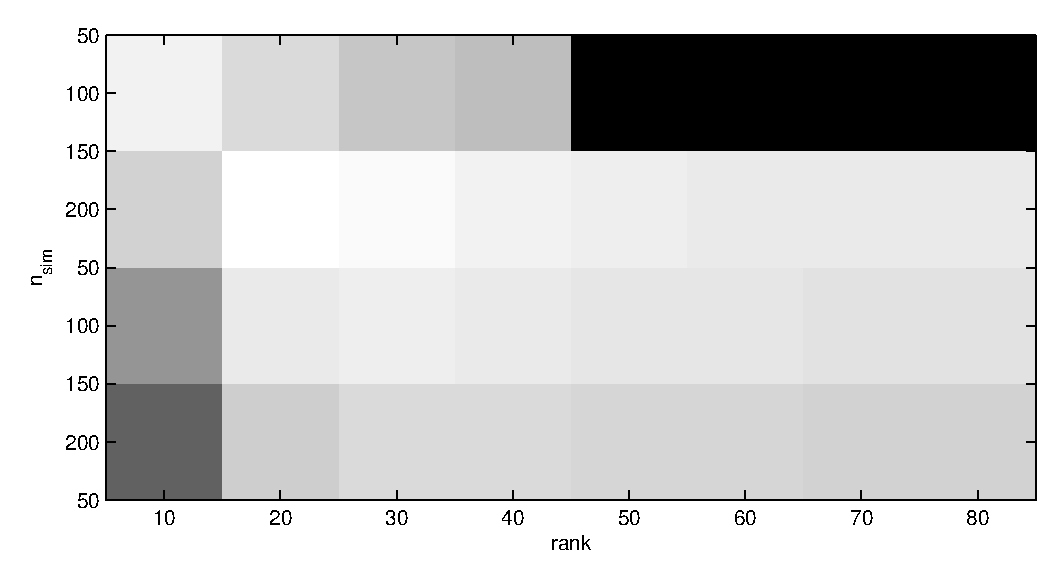
\includegraphics[width=.25\textwidth]{figs/params_tables/psnr_r2-np2-image_s40_average_derf.eps}\\
		\includegraphics[width=.25\textwidth]{figs/params_tables/time_r2-np2-image_s10_average_derf.eps}%
		\includegraphics[width=.25\textwidth]{figs/params_tables/time_r2-np2-image_s20_average_derf.eps}%
		\includegraphics[width=.25\textwidth]{figs/params_tables/time_r2-np2-image_s40_average_derf.eps}\\
	\end{center}
	\caption{Top row: average PSNRs over four sequences, obtained by varying the second stage parameters
		$r$ and $n_{\text{sim}}$. From left to right, results for $\sigma = 10,
		20, 40$. In each image, the contrast has been stretched so that white
		corresponds to the maximum PSNR and black to a decay of 1dB bellow the
		maximum. 
		Bottom: corresponding average running times. White corresponds to $50$ s/frame (using parallelization with four threads).}
	\label{fig:rank-nsim-image-stage2}
\end{figure*}


\begin{figure*}[htpb!]
	\begin{center}
		\includegraphics[width=.25\textwidth]{figs/params_tables/psnr_r1-np1-image_s10_average_derf.eps}%
		\includegraphics[width=.25\textwidth]{figs/params_tables/psnr_r1-np1-image_s20_average_derf.eps}%
		\includegraphics[width=.25\textwidth]{figs/params_tables/psnr_r1-np1-image_s40_average_derf.eps}\\
		\includegraphics[width=.25\textwidth]{figs/params_tables/time_r1-np1-image_s10_average_derf.eps}%
		\includegraphics[width=.25\textwidth]{figs/params_tables/time_r1-np1-image_s20_average_derf.eps}%
		\includegraphics[width=.25\textwidth]{figs/params_tables/time_r1-np1-image_s40_average_derf.eps}\\
	\end{center}
	\caption{Same as Figure \ref{fig:rank-nsim-image-stage2} but for the first stage.}
	\label{fig:rank-nsim-image-stage1}
\end{figure*}








%figs/params_tables/psnr_r1-np1-image_s10_bus.eps
%figs/params_tables/psnr_r1-np1-image_s20_bus.eps
%figs/params_tables/psnr_r1-np1-image_s40_bus.eps
%figs/params_tables/time_r1-np1-image_s10_bus.eps
%figs/params_tables/time_r1-np1-image_s20_bus.eps
%figs/params_tables/time_r1-np1-image_s40_bus.eps


%\begin{figure*}[htpb!]
%	\begin{center}
%		\includegraphics[width=.25\textwidth,height=.19\textwidth]{figs/params_tables/zoom_psnr_px1-np1-bars_1r8_s10_average.eps}%
%		\includegraphics[width=.25\textwidth,height=.19\textwidth]{figs/params_tables/zoom_psnr_px1-np1-bars_1r16_s10_average.eps}%
%		\includegraphics[width=.25\textwidth,height=.19\textwidth]{figs/params_tables/zoom_psnr_px1-np1-bars_1r32_s10_average.eps}%
%		\includegraphics[width=.25\textwidth,height=.19\textwidth]{figs/params_tables/zoom_psnr_px1-np1-bars_1r64_s10_average.eps}\\
%		\includegraphics[width=.25\textwidth,height=.19\textwidth]{figs/params_tables/zoom_psnr_px1-np1-bars_1r8_s20_average.eps}%
%		\includegraphics[width=.25\textwidth,height=.19\textwidth]{figs/params_tables/zoom_psnr_px1-np1-bars_1r16_s20_average.eps}%
%		\includegraphics[width=.25\textwidth,height=.19\textwidth]{figs/params_tables/zoom_psnr_px1-np1-bars_1r32_s20_average.eps}%
%		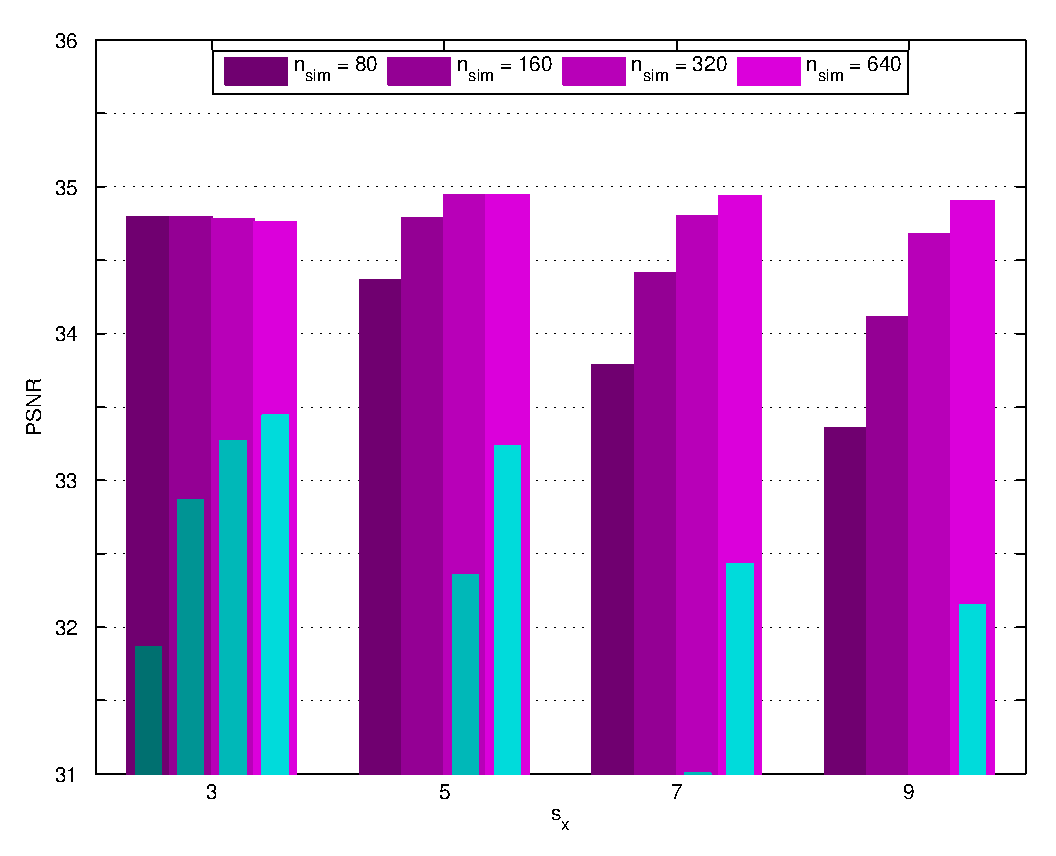
\includegraphics[width=.25\textwidth,height=.19\textwidth]{figs/params_tables/zoom_psnr_px1-np1-bars_1r64_s20_average.eps}\\
%		\includegraphics[width=.25\textwidth,height=.19\textwidth]{figs/params_tables/zoom_psnr_px1-np1-bars_1r8_s40_average.eps}%
%		\includegraphics[width=.25\textwidth,height=.19\textwidth]{figs/params_tables/zoom_psnr_px1-np1-bars_1r16_s40_average.eps}%
%		\includegraphics[width=.25\textwidth,height=.19\textwidth]{figs/params_tables/zoom_psnr_px1-np1-bars_1r32_s40_average.eps}%
%		\includegraphics[width=.25\textwidth,height=.19\textwidth]{figs/params_tables/zoom_psnr_px1-np1-bars_1r64_s40_average.eps}\\
%	\end{center}
%	\caption{Average PSNRs for 64 configurations of the first stage parameters
%		$r$, $n_{\text{sim}}$ and $s_x$. From top to bottom, results for $\sigma = 10, 20, 40$.
%		From left to right: results for $r = 8, 16, 32, 64$.}
%	\label{fig:rank-px-nsim-table-stage1}
%\end{figure*}
%
%\begin{figure*}[htpb!]
%	\begin{center}
%		\includegraphics[width=.25\textwidth,height=.19\textwidth]{figs/params_tables/zoom_psnr_px2-np2-bars_2r8_s10_average.eps}%
%		\includegraphics[width=.25\textwidth,height=.19\textwidth]{figs/params_tables/zoom_psnr_px2-np2-bars_2r16_s10_average.eps}%
%		\includegraphics[width=.25\textwidth,height=.19\textwidth]{figs/params_tables/zoom_psnr_px2-np2-bars_2r32_s10_average.eps}%
%		\includegraphics[width=.25\textwidth,height=.19\textwidth]{figs/params_tables/zoom_psnr_px2-np2-bars_2r64_s10_average.eps}\\
%		\includegraphics[width=.25\textwidth,height=.19\textwidth]{figs/params_tables/zoom_psnr_px2-np2-bars_2r8_s20_average.eps}%
%		\includegraphics[width=.25\textwidth,height=.19\textwidth]{figs/params_tables/zoom_psnr_px2-np2-bars_2r16_s20_average.eps}%
%		\includegraphics[width=.25\textwidth,height=.19\textwidth]{figs/params_tables/zoom_psnr_px2-np2-bars_2r32_s20_average.eps}%
%		\includegraphics[width=.25\textwidth,height=.19\textwidth]{figs/params_tables/zoom_psnr_px2-np2-bars_2r64_s20_average.eps}\\
%		\includegraphics[width=.25\textwidth,height=.19\textwidth]{figs/params_tables/zoom_psnr_px2-np2-bars_2r8_s40_average.eps}%
%		\includegraphics[width=.25\textwidth,height=.19\textwidth]{figs/params_tables/zoom_psnr_px2-np2-bars_2r16_s40_average.eps}%
%		\includegraphics[width=.25\textwidth,height=.19\textwidth]{figs/params_tables/zoom_psnr_px2-np2-bars_2r32_s40_average.eps}%
%		\includegraphics[width=.25\textwidth,height=.19\textwidth]{figs/params_tables/zoom_psnr_px2-np2-bars_2r64_s40_average.eps}\\
%	\end{center}
%	\caption{Average PSNRs for 64 configurations of the second stage parameters
%		$r$, $n_{\text{sim}}$ and $s_x$. From top to bottom, results for $\sigma = 10, 20, 40$.
%		From left to right: results for $r = 8, 16, 32, 64$.}
%	\label{fig:rank-px-nsim-table-stage2}
%\end{figure*}


%For the experiments shown in \S \ref{sec:results} we used the following 
%parameters.
%\begin{LaTeXdescription}
%	\item[Patch size:] In both stages, we fixed the patch size at $s = 5$. Better 
%		results can be obtained with higher patch sizes, but the computational cost
%		scales considerably (e.g. the inversion of the covariance matrix is of $O(s^6)$).
%	\item[Number of similar patches:] For the first stage, we set
%		$N^{(1)}_{\text{sim}} = 3s^2n_t$  (recall that $n_t$ is the temporal
%		extend of the search region). For the second step we 
%		found better results using fewer patches, thus we set $N^{(2)}_{\text{sim}} = 3/4 s^2n_t$.
%	\item[Search region:] In both stages, we used $n_x = s^2/2$.
%		For the temporal search region, we found a good trade-off
%		between computational time and quality of the results for $n_t = 5$. 
%	\item[Patch distance threshold:] When building the group of similar patches
%		in the second stage, more than $N_{\text{sim}}$ patches are allowed if their 
%		distances with respect to the reference patch are smaller than a threshold $\tau$.
%		As in \cite{Lebrun2013ipol}, we set $\tau = 4$ (the distance between patches is normalized by 
%		the number of elements in the patch and the number of channels).
%\end{LaTeXdescription}

% stage 1
%
% patch size $s = 5$
% spatial search region $n_x = 37$
% temporal search region $n_t = 0,3,5$
% number of similar patches $3 s^2 n_t$, 3/4 s^2 n_t$$
% beta $\beta = 1; 1.2$
% tau n/a $\tau = 16$  
% offset $= s/2$

% stage 2
%
% patch size 
% spatial search region
% temporal search region
% number of similar patches
% beta
% tau
% offset

\begin{table*}[htp!]
	\begin{center}
		{%\small
		\renewcommand{\tabcolsep}{1.6mm}
		\renewcommand{\arraystretch}{1.3}
		\begin{tabular}{ c | l |c c | c c | c c | c c | c c | c c}
			\hline
			\rule{0pt}{10pt}$\sigma$ & Method            & \multicolumn{2}{c}{Tennis}  & \multicolumn{2}{c}{Coastguard}&\multicolumn{2}{c}{Foreman}& \multicolumn{2}{c}{Bus}     &\multicolumn{2}{c|}{Football}& \multicolumn{2}{c}{Average}\\\hline
			\multirow{1}{*}{$ 5$}
%			                      & CIFIC                & \bsic{     } &              & \bsic{     } &              & \bsic{     } &              & \bsic{     } &              & \bsic{     } &              & \bsic{     } &              \\
			                      & V-BM3D               & \bsic{     } &       39.45  & \bsic{     } &       40.18  & \bsic{     } &       40.16  & \bsic{     } &       39.07  & \bsic{     } &              & \bsic{     } &              \\
			                      & V-BM4D-tip           & \bsic{     } & \best{39.98} & \bsic{     } & \best{41.13} & \bsic{     } & \best{41.38} & \bsic{     } & \best{40.21} & \bsic{     } & \best{     } & \bsic{     } & \best{     } \\
			                      & V-BM4D-mp            & \bsic{39.61} &       39.60  & \bsic{40.20} &       40.28  & \bsic{40.73} &       40.78  & \bsic{39.45} &       39.56  & \bsic{39.91} &       40.00  & \bsic{todo } &       todo   \\
			                      & VNLB   $s_t = 1$     & \bsic{38.73} &       39.26  & \bsic{40.90} &       41.38  & \bsic{41.19} &       41.82  & \bsic{39.85} &       40.32  & \bsic{41.10} &       41.64  & \bsic{todo } &       todo   \\
			                      & VNLB   $s_t = 2$     & \bsic{39.56} &       40.05  & \bsic{41.61} &       42.08  & \bsic{41.75} &       42.42  & \bsic{40.10} &       40.73  & \bsic{41.29} &       41.88  & \bsic{todo } &       todo   \\
			                      & VNLB   $s_t = 3$     & \bsic{39.82} &       40.16  & \Bsic{41.75} &       42.39  & \Bsic{41.85} &       42.57  & \Bsic{40.16} &       40.96  & \Bsic{41.27} &       41.85  & \Bsic{todo } &       todo   \\
			                      & VNLB   $s_t = 4$     & \Bsic{39.92} & \Best{40.03} & \Bsic{41.76} & \Best{42.41} & \Bsic{41.84} & \Best{42.48} & \Bsic{40.18} & \Best{40.92} & \Bsic{41.23} & \Best{41.67} & \Bsic{todo } & \Best{todo } \\\hline
%                                                                                                                                                                                                                                         
			\multirow{1}{*}{$10$}
%			                      & CIFIC                & \bsic{     } &              & \bsic{     } &              & \bsic{     } &              & \bsic{     } &              & \bsic{     } &              & \bsic{     } &              \\
			                      & V-BM3D               & \bsic{     } &       36.04  & \bsic{     } &       36.82  & \bsic{     } &       37.52  & \bsic{     } &       34.96  & \bsic{     } &              & \bsic{     } &              \\
			                      & V-BM4D-tip           & \bsic{     } & \best{36.42} & \bsic{     } & \best{37.27} & \bsic{     } &       37.92  & \bsic{     } &       36.23  & \bsic{     } &              & \bsic{     } &              \\
			                      & V-BM4D-mp            & \bsic{35.64} &       35.90  & \bsic{36.06} &       36.30  & \bsic{36.96} &       37.21  & \bsic{35.10} &       35.38  & \bsic{35.79} &       36.08  & \bsic{todo } &       todo   \\
			                      & VNLB   $s_t = 1$     & \bsic{34.54} &       35.16  & \bsic{36.81} &       37.23  & \bsic{37.25} &       38.01  & \bsic{35.47} &       36.21  & \bsic{36.88} &       37.69  & \bsic{todo } &       todo   \\
			                      & VNLB   $s_t = 2$     & \bsic{35.67} &       36.28  & \bsic{37.42} &       38.10  & \Bsic{37.87} &       38.82  & \Bsic{35.82} &       36.69  & \Bsic{37.11} &       38.02  & \Bsic{todo } &       todo   \\
			                      & VNLB   $s_t = 3$     & \bsic{35.94} &       36.61  & \Bsic{37.56} &       38.50  & \Bsic{37.93} &       39.08  & \Bsic{35.88} &       36.98  & \Bsic{37.03} &       38.08  & \Bsic{todo } &       todo   \\
			                      & VNLB   $s_t = 4$     & \Bsic{36.02} & \Best{36.73} & \Bsic{37.50} & \Best{38.64} & \Bsic{37.83} & \Best{39.12} & \Bsic{35.87} & \Best{37.11} & \Bsic{36.91} & \Best{38.03} & \Bsic{todo } & \Best{todo } \\\hline
%                                                                                                                                                                                                                                         
			\multirow{1}{*}{$15$}
			                      & CIFIC                & \bsic{     } &       32.76  & \bsic{     } &              & \bsic{     } &              & \bsic{     } &       33.47  & \bsic{     } &       31.59  & \bsic{     } &              \\
%			                      & V-BM3D               & \bsic{     } &              & \bsic{     } &              & \bsic{     } &              & \bsic{     } &              & \bsic{     } &              & \bsic{     } &              \\
%			                      & V-BM4D-tip           & \bsic{     } & \best{     } & \bsic{     } & \best{     } & \bsic{     } & \best{     } & \bsic{     } & \best{     } & \bsic{     } & \best{     } & \bsic{     } & \best{     } \\
			                      & V-BM4D-mp            & \bsic{33.10} &       33.67  & \bsic{33.66} &       34.05  & \bsic{34.78} &       35.17  & \bsic{32.59} &       33.02  & \bsic{33.34} &       33.82  & \bsic{todo } &       todo   \\
			                      & VNLB   $s_t = 1$     & \bsic{32.31} &       32.94  & \bsic{34.32} &       34.95  & \bsic{35.06} &       35.97  & \bsic{33.04} &       33.83  & \bsic{34.62} &       35.50  & \bsic{todo } &       todo   \\
			                      & VNLB   $s_t = 2$     & \bsic{33.36} &       34.12  & \bsic{35.24} &       36.03  & \bsic{35.74} &       36.82  & \bsic{33.39} &       34.29  & \bsic{34.83} &       35.83  & \bsic{todo } &       todo   \\
			                      & VNLB   $s_t = 3$     & \bsic{33.59} &       34.58  & \Bsic{35.33} &       36.38  & \Bsic{35.74} &       37.05  & \Bsic{33.42} &       34.57  & \Bsic{34.72} &       35.88  & \Bsic{todo } &       todo   \\
			                      & VNLB   $s_t = 4$     & \Bsic{33.64} & \Best{34.78} & \Bsic{35.21} & \Best{36.52} & \Bsic{35.57} & \Best{37.11} & \Bsic{33.37} & \Best{34.76} & \Bsic{34.54} & \Best{35.86} & \Bsic{todo } & \Best{todo } \\\hline
%                                                                                                                                                                                                                                         
			\multirow{1}{*}{$20$}
%			                      & CIFIC                & \bsic{     } &              & \bsic{     } &              & \bsic{     } &              & \bsic{     } &              & \bsic{     } &              & \bsic{     } &              \\
			                      & V-BM3D               & \bsic{     } &       32.54  & \bsic{     } &       33.39  & \bsic{     } &       34.49  & \bsic{     } &       31.03  & \bsic{     } &              & \bsic{     } &              \\
			                      & V-BM4D-tip           & \bsic{     } & \best{32.88} & \bsic{     } & \best{33.61} & \bsic{     } & \best{34.62} & \bsic{     } & \best{32.27} & \bsic{     } & \best{     } & \bsic{     } & \best{     } \\
			                      & V-BM4D-mp            & \bsic{31.33} &       31.98  & \bsic{31.91} &       32.44  & \bsic{33.16} &       33.70  & \bsic{30.81} &       31.34  & \bsic{31.58} &       32.22  & \bsic{todo } &       todo   \\
			                      & VNLB   $s_t = 1$     & \bsic{30.78} &       31.38  & \bsic{32.95} &       33.45  & \bsic{33.71} &       34.37  & \bsic{31.60} &       32.19  & \bsic{33.20} &       33.85  & \bsic{todo } &       todo   \\
			                      & VNLB   $s_t = 2$     & \bsic{32.13} &       32.69  & \bsic{33.98} &       34.36  & \bsic{34.55} &       35.41  & \bsic{32.13} &       32.80  & \bsic{33.52} &       34.27  & \bsic{todo } &       todo   \\
			                      & VNLB   $s_t = 3$     & \bsic{32.53} &       33.12  & \Bsic{34.14} &       34.74  & \Bsic{34.69} &       35.75  & \Bsic{32.27} &       33.13  & \Bsic{33.50} &       34.35  & \Bsic{todo } &       todo   \\
			                      & VNLB   $s_t = 4$     & \Bsic{32.67} & \Best{33.32} & \Bsic{34.13} & \Best{34.92} & \Bsic{34.60} & \Best{35.86} & \Bsic{32.31} & \Best{33.34} & \Bsic{33.41} & \Best{34.34} & \Bsic{todo } & \Best{todo } \\\hline
%                                                                                                                                                                                                                                         
			\multirow{1}{*}{$25$}
			                      & CIFIC                & \bsic{     } &       29.74  & \bsic{     } &              & \bsic{     } &              & \bsic{     } &       30.48  & \bsic{     } &       28.82  & \bsic{     } &              \\
%			                      & V-BM3D               & \bsic{     } &              & \bsic{     } &              & \bsic{     } &              & \bsic{     } &              & \bsic{     } &              & \bsic{     } &              \\
%			                      & V-BM4D-tip           & \bsic{     } & \best{     } & \bsic{     } & \best{     } & \bsic{     } & \best{     } & \bsic{     } & \best{     } & \bsic{     } & \best{     } & \bsic{     } & \best{     } \\
			                      & V-BM4D-mp            & \bsic{30.01} &       30.73  & \bsic{30.60} &       31.24  & \bsic{31.91} &       32.59  & \bsic{29.46} &       30.07  & \bsic{30.22} &       30.96  & \bsic{todo } &       todo   \\
			                      & VNLB   $s_t = 1$     & \bsic{29.67} &       30.27  & \bsic{31.51} &       32.18  & \bsic{32.43} &       33.30  & \bsic{30.39} &       30.95  & \bsic{31.92} &       32.74  & \bsic{todo } &       todo   \\
			                      & VNLB   $s_t = 2$     & \bsic{30.88} &       31.57  & \bsic{32.79} &       33.40  & \bsic{33.46} &       34.30  & \bsic{30.89} &       31.50  & \bsic{32.34} &       33.16  & \bsic{todo } &       todo   \\
			                      & VNLB   $s_t = 3$     & \bsic{31.30} &       32.05  & \Bsic{33.00} &       33.73  & \Bsic{33.60} &       34.61  & \Bsic{31.01} &       31.83  & \Bsic{32.32} &       33.22  & \Bsic{todo } &       todo   \\
			                      & VNLB   $s_t = 4$     & \Bsic{31.44} & \Best{32.30} & \Bsic{32.97} & \Best{33.88} & \Bsic{33.51} & \Best{34.73} & \Bsic{31.02} & \Best{32.05} & \Bsic{32.20} & \Best{33.21} & \Bsic{todo } & \Best{todo } \\\hline
%                                                                                                                                                                                                                                         
			\multirow{1}{*}{$40$}
%			                      & CIFIC                & \bsic{     } &              & \bsic{     } &              & \bsic{     } &              & \bsic{     } &              & \bsic{     } &              & \bsic{     } &              \\
			                      & V-BM3D               & \bsic{     } &       29.20  & \bsic{     } & \best{29.99} & \bsic{     } &       31.17  & \bsic{     } &       27.34  & \bsic{     } &              & \bsic{     } &              \\
			                      & V-BM4D-tip           & \bsic{     } & \best{29.52} & \bsic{     } & \best{30.00} & \bsic{     } & \best{31.30} & \bsic{     } &       28.32  & \bsic{     } &              & \bsic{     } &              \\
			                      & V-BM4D-mp            & \bsic{27.34} &       28.14  & \bsic{27.81} &       28.73  & \bsic{29.01} &       30.09  & \bsic{26.67} &       27.44  & \bsic{27.45} &       28.35  & \bsic{todo } &       todo   \\
			                      & VNLB   $s_t = 1$     & \bsic{27.17} &       28.04  & \bsic{28.80} &       29.72  & \bsic{29.72} &       30.85  & \bsic{27.64} &       28.32  & \bsic{29.13} &       30.11  & \bsic{todo } &       todo   \\
			                      & VNLB   $s_t = 2$     & \bsic{28.43} &       29.38  & \bsic{30.16} &       31.03  & \bsic{30.84} &       32.09  & \bsic{28.21} &       29.07  & \bsic{29.63} &       30.67  & \bsic{todo } &       todo   \\
			                      & VNLB   $s_t = 3$     & \Bsic{28.84} &       29.83  & \Bsic{30.40} &       31.32  & \Bsic{30.99} &       32.50  & \Bsic{28.31} &       29.38  & \Bsic{29.64} &       30.76  & \Bsic{todo } &       todo   \\
			                      & VNLB   $s_t = 4$     & \Bsic{28.97} & \Best{30.05} & \Bsic{30.36} & \Best{31.45} & \Bsic{30.89} & \Best{32.65} & \Bsic{28.29} & \Best{29.57} & \Bsic{29.52} & \Best{30.76} & \Bsic{todo } & \Best{todo } \\\hline
		\end{tabular}}
	\end{center}
% Command to print rounded psnrs
% for i in $(cat bus_s40_pt*/measures | grep PSNR_final | sed "s/^-PSNR_final\ =\ "//); do  echo "scale=2;(((10^2)*$i)+0.5)/(10^2)" | bc; done
	\caption{PSNRs obtained for the four classic color test sequences used in
	\cite{Maggioni2012}. See text for details.}
	\label{tab:psnr-classic-color}
\end{table*}

\begin{table*}[htp!]
	\begin{center}
		{\small
		\renewcommand{\tabcolsep}{1.6mm}
		\renewcommand{\arraystretch}{1.3}
		\begin{tabular}{ c | l |c c | c c | c c | c c | c c | c c | c c}
			\hline
			\rule{0pt}{6pt}$\sigma$ & Method             & \multicolumn{2}{c}{Tennis}  & \multicolumn{2}{c}{Salesman} &\multicolumn{2}{c}{Fl. garden}& \multicolumn{2}{c}{Mobile}  & \multicolumn{2}{c}{Bicycle}  & \multicolumn{2}{c|}{Stefan} & \multicolumn{2}{c}{Average} \\\hline
			\multirow{1}{*}{$10$}
			                      & LZD                  & \bsic{     } & \Best{36.45} & \bsic{     } & \Best{40.49}  & \bsic{     } & \Best{34.46}  & \bsic{     } & \Best{37.03} &              &               &              &              & \bsic{     } &       37.13  \\
			                      & V-BM4D-tip           & \bsic{     } &       35.22  & \bsic{     } &       37.30   & \bsic{     } &       32.81   &              &              &              &       37.66   &              &              & \bsic{     } &       35.11  \\
			                      & V-BM4D-mp            & \Bsic{34.32} &       34.95  & \Bsic{36.77} &       37.48   & \bsic{32.20} &       32.01   & \bsic{33.99} &       34.11  & \Bsic{37.58} &       37.85   & \bsic{33.47} &       33.68  & \bsic{todo } &       todo   \\
			                      & VNLB   $s_t = 1$     & \bsic{32.99} &       33.29  & \bsic{34.62} &       35.15   & \bsic{30.80} &       31.22   & \bsic{32.34} &       32.79  & \bsic{36.21} &       37.72   & \bsic{33.20} &       33.79  & \bsic{todo } &       todo   \\
										 & VNLB   $s_t = 2$     & \Bsic{34.35} &       34.68  & \bsic{35.87} &       36.62   & \bsic{32.41} &       32.92   & \Bsic{34.26} &       34.78  & \bsic{36.86} & \Best{38.55}  & \Bsic{33.73} & \Best{34.38} & \Bsic{todo } &       todo   \\
										 & VNLB   $s_t = 3$     & \Bsic{34.34} &       35.23  & \bsic{35.63} &       37.08   & \bsic{32.39} &       33.18   & \bsic{34.02} &       35.25  & \bsic{36.57} & \Best{38.45}  & \bsic{33.45} & \Best{34.36} & \bsic{todo } &       todo   \\
			                      & VNLB   $s_t = 4$     & \Bsic{34.25} &       35.40  & \bsic{35.39} &       37.21   & \Bsic{32.54} &       33.10   & \bsic{34.03} &       35.48  & \bsic{36.05} &       38.27   & \bsic{33.39} &       34.10  & \bsic{todo } &       todo   \\\hline
%			                      & VNLB   $s_t = 2$     & \bsic{34.33} &       34.62  & \Bsic{todo } &       todo    & \Bsic{todo } &       todo    & \bsic{34.44} &       34.67  & \Bsic{todo } &       todo    & \Bsic{33.82} & \Best{34.23} & \Bsic{todo } &       todo   \\
%			                      & VNLB   $s_t = 3$     & \Bsic{34.53} &       35.15  & \bsic{todo } & \Best{todo }  & \bsic{todo } & \Best{todo }  & \Bsic{34.74} &       35.31  & \bsic{todo } & \Best{todo }  & \Bsic{33.81} & \Best{34.29} & \bsic{todo } &       todo   \\
%			                      & VNLB   $s_t = 4$     & \bsic{34.18} & \Best{35.32} & \bsic{todo } &       todo    & \bsic{todo } &       todo    & \bsic{34.41} & \Best{35.54} & \bsic{todo } &       todo    & \bsic{33.47} &       34.13  & \bsic{todo } &       todo   \\\hline
%                                                                                                                                                                                                                                                                         
			\multirow{1}{*}{$20$}                                                                                                                                                                                                                                            
			                      & LZD                  & \bsic{     } & \Best{33.36} & \bsic{     } & \Best{37.52}  & \bsic{     } & \Best{31.35}  & \bsic{     } & \Best{33.47} &              &               &              &              & \bsic{     } &       34.08  \\
			                      & V-BM4D-tip           & \bsic{     } &       31.59  & \bsic{     } &       33.79   & \bsic{     } &       28.63   &              &              &              &       34.10   &              &              & \bsic{     } &       31.34  \\
			                      & V-BM4D-mp            & \bsic{30.54} &       31.08  & \Bsic{32.18} &       33.46   & \Bsic{28.12} &       28.32   & \Bsic{29.67} &       30.49  & \Bsic{33.62} &       34.54   & \bsic{29.04} &       29.69  & \bsic{todo } &       todo   \\
			                      & VNLB   $s_t = 1$     & \bsic{29.62} &       30.16  & \bsic{30.76} &       31.54   & \bsic{26.17} &       26.56   & \bsic{27.89} &       28.39  & \bsic{32.41} &       33.77   & \bsic{28.69} &       29.26  & \bsic{todo } &       todo   \\
										 & VNLB   $s_t = 2$     & \Bsic{30.81} &       31.37  & \bsic{31.98} &       33.08   & \bsic{27.89} &       28.41   & \Bsic{29.69} &       30.41  & \bsic{33.17} & \Best{34.97}  & \Bsic{29.32} & \Best{30.00} & \Bsic{todo } &       todo   \\
			                      & VNLB   $s_t = 3$     & \bsic{29.88} &       31.62  & \bsic{30.60} &       33.05   & \bsic{27.50} &       28.89   & \bsic{29.02} &       30.86  & \bsic{31.23} &       34.26   & \bsic{28.51} & \Best{30.08} & \bsic{todo } &       todo   \\
			                      & VNLB   $s_t = 4$     & \bsic{29.49} &       31.64  & \bsic{30.10} &       32.94   & \bsic{27.47} &       29.07   & \bsic{28.86} &       31.12  & \bsic{30.51} &       33.88   & \bsic{28.26} & \Best{30.03} & \bsic{todo } &       todo   \\\hline
%			                      & VNLB   $s_t = 2$     & \Bsic{30.73} &       31.24  & \Bsic{todo } & \Best{todo }  & \Bsic{todo } & \Best{todo }  & \bsic{29.83} &       30.34  & \Bsic{todo } & \Best{todo }  & \Bsic{29.38} &       29.90  & \Bsic{todo } &       todo   \\
%			                      & VNLB   $s_t = 3$     & \Bsic{30.82} &       31.66  & \bsic{todo } & \Best{todo }  & \bsic{todo } & \Best{todo }  & \Bsic{30.15} &       31.09  & \bsic{todo } & \Best{todo }  & \Bsic{29.33} & \Best{30.02} & \bsic{todo } &       todo   \\
%			                      & VNLB   $s_t = 4$     & \bsic{30.25} & \Best{31.69} & \bsic{todo } &       todo    & \bsic{todo } &       todo    & \bsic{29.74} & \Best{31.35} & \bsic{todo } &       todo    & \bsic{28.89} & \Best{29.97} & \bsic{todo } &       todo   \\\hline
%                                                                                                                                                                                                                                                                         
			\multirow{1}{*}{$30$}                                                                                                                                                                                                                                            
			                      & LZD                  & \bsic{     } & \Best{31.62} & \bsic{     } & \Best{36.05}  & \bsic{     } & \Best{29.09}  & \bsic{     } & \Best{30.36} &              &               &              &              & \bsic{     } &       32.25  \\
			                      & V-BM4D-tip           & \bsic{     } &       29.72  &              &       31.75   & \bsic{     } &       26.29   &              &              &              &       31.83   &              &              & \bsic{     } &       29.25  \\
			                      & V-BM4D-mp            & \Bsic{28.89} &       29.37  & \Bsic{29.56} &       31.02   & \Bsic{25.63} &       26.20   & \bsic{26.73} &       27.99  & \Bsic{30.99} &       32.30   & \bsic{26.39} &       27.34  & \bsic{todo } &       todo   \\
			                      & VNLB   $s_t = 1$     & \bsic{27.32} &       28.20  & \bsic{27.94} &       29.14   & \bsic{23.62} &       23.96   & \bsic{25.42} &       25.82  & \bsic{29.50} &       31.08   & \bsic{26.14} &       26.69  & \bsic{todo } &       todo   \\
										 & VNLB   $s_t = 2$     & \bsic{28.65} &       29.51  & \Bsic{29.55} &       30.93   & \bsic{25.33} &       25.78   & \Bsic{27.31} &       27.90  & \bsic{30.70} & \Best{32.63}  & \Bsic{26.99} &       27.55  & \Bsic{todo } &       todo   \\
										 & VNLB   $s_t = 3$     & \bsic{27.49} &       29.71  & \bsic{27.91} &       30.91   & \bsic{24.75} &       26.36   & \bsic{26.30} &       28.43  & \bsic{28.45} &       31.95   & \bsic{25.95} & \Best{27.72} & \bsic{todo } &       todo   \\
			                      & VNLB   $s_t = 4$     & \bsic{26.92} &       29.64  & \bsic{27.28} &       30.73   & \bsic{24.60} &       26.60   & \bsic{26.04} &       28.68  & \bsic{27.61} &       31.50   & \bsic{25.57} & \Best{27.71} & \bsic{todo } &       todo   \\\hline
%                                                                                                                                                                                                                                                                         
			\multirow{1}{*}{$40$}                                                                                                                                                                                                                                            
			                      & LZD                  & \bsic{     } & \Best{30.79} & \bsic{     } & \Best{35.12}  & \bsic{     } & \Best{27.56}  & \bsic{     } & \Best{28.93} &              &               &              &              & \bsic{     } &       31.16  \\
			                      & V-BM4D-tip           & \bsic{     } &       28.49  & \bsic{     } &       30.35   & \bsic{     } &       24.60   &              &              &              &       30.10   &              &              & \bsic{     } &       27.81  \\
			                      & V-BM4D-mp            & \Bsic{27.67} &       28.38  & \Bsic{27.81} &       29.37   & \Bsic{23.68} &       24.59   & \bsic{24.64} &       26.02  & \Bsic{29.02} &       30.58   & \bsic{24.47} &       25.64  & \bsic{todo } &       todo   \\
			                      & VNLB   $s_t = 1$     & \bsic{25.65} &       26.83  & \bsic{25.97} &       27.49   & \bsic{21.89} &       22.25   & \bsic{23.57} &       24.11  & \bsic{27.32} &       29.03   & \bsic{24.27} &       24.97  & \bsic{todo } &       todo   \\
										 & VNLB   $s_t = 2$     & \bsic{27.09} &       28.27  & \bsic{27.67} &       29.46   & \bsic{23.56} &       24.06   & \Bsic{25.48} &       26.17  & \bsic{28.64} & \Best{30.90}  & \Bsic{25.21} &       25.89  & \bsic{todo } &       todo   \\
										 & VNLB   $s_t = 3$     & \bsic{25.66} &       28.33  & \bsic{25.93} &       29.31   & \bsic{22.84} &       24.65   & \bsic{24.35} &       26.69  & \bsic{26.31} &       30.11   & \bsic{24.11} & \Best{26.08} & \Bsic{todo } &       todo   \\
			                      & VNLB   $s_t = 4$     & \bsic{24.98} &       28.16  & \bsic{25.18} &       29.03   & \bsic{22.62} &       24.89   & \bsic{23.98} &       26.90  & \bsic{25.41} &       29.59   & \bsic{23.64} & \Best{26.05} & \Bsic{todo } &       todo   \\\hline
%			                      & VNLB   $s_t = 2$     & \bsic{27.14} &       28.15  & \bsic{todo } &       todo    & \bsic{todo } &       todo    & \bsic{25.43} &       26.06  & \bsic{todo } &       todo    & \bsic{25.18} &       25.81  & \bsic{todo } &       todo   \\
%			                      & VNLB   $s_t = 3$     & \bsic{27.63} &       28.62  & \Bsic{todo } & \Best{todo }  & \Bsic{todo } & \Best{todo }  & \bsic{26.15} &       26.94  & \Bsic{todo } & \Best{todo }  & \Bsic{25.44} & \Best{26.12} & \Bsic{todo } & \Best{todo } \\
%			                      & VNLB   $s_t = 4$     & \Bsic{27.81} & \Best{28.86} & \Bsic{todo } & \Best{todo }  & \Bsic{todo } & \Best{todo }  & \Bsic{26.45} & \Best{27.46} & \Bsic{todo } & \Best{todo }  & \Bsic{25.50} & \Best{26.24} & \Bsic{todo } & \Best{todo } \\\hline
		\end{tabular}}
% Command to print rounded psnrs
% for i in $(cat bus_s40_pt*/measures | grep PSNR_final | sed "s/^-PSNR_final\ =\ "//); do  echo "scale=2;(((10^2)*$i)+0.5)/(10^2)" | bc; done
	\end{center}
	\caption{Quantitative denoising results for some classic grayscale test sequences. See text for details.}
	\label{tab:psnr-classic-gray}
\end{table*}

%\begin{table*}[htp!]
%	\begin{center}
%	\renewcommand{\tabcolsep}{2mm}
%	\renewcommand{\arraystretch}{1.0}
%	\begin{tabular}{ c | l |c c c c c}
%		\hline
%		\rule{0pt}{12pt}$\sigma$ & Method     & Army & DogDance & Evergreen & Mequon & Walking  \\\hline
%		\multirow{5}{*}{$10$} & V-BM4D-np      &       37.77  &       35.70  &       35.40  &       38.09  &       38.85  \\
%		                      & VNLB $n_t = 0$ &       36.90  &       35.42  &       34.84  &       38.43  &       38.86  \\
%		                      & VNLB $n_t = 3$ &       37.65  &       35.87  &       35.38  &       39.09  &       39.69  \\
%									 & VNLB $n_t = 5$ & \best{37.88} & \best{36.01} & \best{35.53} & \best{39.20} & \best{39.74} \\\hline
%%									                                                                                           
%		\multirow{5}{*}{$20$} & V-BM4D-np      &       32.91  &       31.50  &       30.94  &       33.60  &       34.27  \\
%		                      & VNLB $n_t = 0$ &       33.77  &       32.44  &       31.68  &       35.61  &       35.60  \\
%									 & VNLB $n_t = 3$ &       34.45  &       32.90  &       32.15  &       35.89  &       36.12  \\
%									 & VNLB $n_t = 5$ & \best{34.59} & \best{33.02} & \best{32.27} & \best{35.90} & \best{36.12} \\\hline
%%									                                                                                           
%		\multirow{5}{*}{$40$} & V-BM4D-np      &       30.42  &       29.29  &       28.65  &       31.02  &       31.64  \\
%		                      & VNLB $n_t = 0$ &       30.55  &       29.41  &       28.66  &       31.78  &       31.86  \\
%									 & VNLB $n_t = 3$ & \best{31.02} & \best{29.73} & \best{29.03} & \best{31.88} & \best{31.92} \\
%									 & VNLB $n_t = 5$ & \best{31.06} & \best{29.74} & \best{29.08} &       31.70  &       31.74  \\\hline
%	\end{tabular}
%	\end{center}
%	\caption{PSNRs obtained for the five color sequences from the Middlebury
%	dataset \cite{middleburyOflow}. See text for details.}
%	\label{tab:psnr-middlebury}
%\end{table*}

\section{Results}
\label{sec:results}

In this section we present results obtained with the proposed
method on some classic test sequences with Gaussian noise added.
We consider separatedly the cases of grayscale and color videos.

\subsection{Results on grayscale videos}

We present denoising results on six classic test sequences used commonly in the
literature. We compare against two state-of-the-art methods: V-BM4D
\cite{Maggioni2012}, and the method of Li, Zhang and Dai \cite{LiZhangDai2011}
which we call I-SA-BM4D, since it can be regarded as an iterative version of BM4D \cite{Maggioni2013}
using shape adaptive 3D patches, as in \todo{REF}.  
For V-BM4D, we show results corresponding to two
different choices of parameters. The method labeled V-BM4D-tip
corresponds to the results reported
in \cite{Maggioni2012}. The results labeled V-BM4D-mp were
obtained using the implementation available online \cite{bm4dcode}. This
implementation provides three parameter profiles of increasing quality and
complexity: ``low complexity profile'', ``normal profile'' and ``modified
profile''. We show the results obtained with the modified profile.

Each sequence was contaminated with white Gaussian noise of $\sigma =
10,20,30,40$. Table \ref{tab:psnr-classic-gray} shows the
PSNR values obtained after denoising. For our method, we show results varying the temporal
component of the patch size between $1$ (2D patch) and $4$ frames.
For our method and V-BM4D-mp we show the PSNR of the basic estimate as well.

The best results by a large margin are the ones reported in
\cite{LiZhangDai2011}. This method builds uppon BM4D, which in \cite{Maggioni2013}
is applied to volumetric imagery. In this work, its applicability to video is
also explored, and the results show that it is inferior to V-BM4D, at least 
for moderate noise levels. The method of Li, Zhang and Dai \cite{LiZhangDai2011} 
considers shape adaptive patches, and also several iterations (in each iteration,
the previous iterate is used as an oracle to compute patch distances and the
signal energy in the Wiener filtering step) \todo{Check this}. It seems that both elements
contribute to achieve this significant difference.

We can see that our results are comarable with the ones of V-BM4D. \todo{We need to find new parameters
for grayscale sequences. This discussion needs to be rewritten based on the updated results.}


\subsection{Results on color videos}

We considered five color test sequences, \emph{tennis}, \emph{coastguard},
\emph{foreman}, \emph{bus} and \emph{football}. The first four were chosen
because they were used in \cite{Maggioni2012}. The fifth one, \emph{football},
was added to test the performance of our method on a sequence with complex motions.

We compared our method with CIFIC \cite{Dai2013} and V-BM4D \cite{Maggioni2012}, two recent
state-of-the-art methods. As with grayscale videos, for V-BM4D, we show results corresponding to two
different parameter configurations: V-BM4D-tip
corresponds to the results reported
in \cite{Maggioni2012}, and V-BM4D-mp corresponds to the ``modified profile''
of the implementation available online \cite{bm4dcode}.

Let us note that the modified profile has a
computation time lower to that of our method. Running with a
single core in a Intel Xeon X7560 (2.27GHz) CPU, 
our current implementation takes on average $XXs$ per frame for a video of CIF
resolution ($352\times288$). V-BM4D takes $44s$ with the modified profile.
\todo{Compute running times!!!}

The results are shown in Table \ref{tab:psnr-classic}. The proposed method is
labeled VNLB. It achieves the highest PSNR values on all the considered
sequences and levels of noise, with a significant difference. The difference
increases for higher levels of noise. A possible reason for this is that both 
CIFIC and V-BM4D rely on motion estimation by 2D block matching, which might
not be reliable for high noise levels.

%We also show quantitative results obtained in for some sequences from the
%optical flow Middlebury dataset (the sequences have 8 frames each), and compare
%against V-BM4D-np (see table \ref{tab:psnr-middlebury}. For these sequences, the
%proposed method outpeforms V-BM4D-np.

For a qualitative analysis we show in Figure \ref{fig:results} results obtained
with nonlocal Bayes (setting $n_t = 5$) and V-BM4D-np. Interestingly, for $\sigma = 20$
and $40$, V-BM4D-np is able to better recover the wallpaper texture in tennis,
but does worse than VNLB for the foliage texture of the trees in bus. 
%One
%plausible reason for this is that the spatial bi-orthogonal wavelets and
%DCT transforms used by BM4D are very well suited to the structured pattern of the
%wallpaper.
For high levels of noise, the wallpaper texture is masked by the noise. 
It is possible that when comparing 2D patches the noise dominates in the
comparison. Using spatio-temporal volumes reduces the distance noise,
allowing to find similar patches with the same regular texture pattern.

\subsection{Evaluating temporal consistency}

An important aspect of the quality of any video processing algorithm is the 
temporal consistency of the result. Similar to previous works \cite{Liu2010, Sutour2014}
we evaluate quantitatively the temporal consistency of our denoising results.
To that aim run VNLB and V-BM4D-mp on four sequences of MPI Sintel's training
dataset. These are CGI color sequences with ground truth forward optical flow, which we
denote by $v:\Omega\times\{1,\dots,T-1\}\rightarrow \mathds R^2$. 
The forward optical flow $v(x,t)$ encodes the motion displacement of pixel $x$
between frames $t$ and $t +1$.
We use the optical flow to evaluate the variations along motion trajectories
added by the denoising algorithm. To that aim we estimate the derivative along
motion trajectories of the denoising error $e = \widetilde u - u$ as follows:
\[\partial_v e(x,t) =
\left\{
\begin{array}{l l}
	e(x + v(x,t), t+1) - e(x,t), & \text{if } (x,t)\not\in \mathcal{K},\\
	0 & \text{if } (x,t)\in \mathcal{K}.
\end{array}
\right.\]
Here $\mathcal K$ is the set of pixels that are occluded or escape out of the video
domain. The occlusion set $\mathcal K$ is also provided in MPI Sintel's database.
Note that since the optical flow is sub-pixelic, the value of $e(x + v(x,t),t+1)$
needs to be interpolated. We use bilinear interpolation.

We define a temporal consistency error as follows:
\[\text{TCE} = 10 \log_{10}\left(\frac{255^2 c|\Omega|T}{\|\partial_v e\|_2^2}\right)\]
where $\|\,\cdot\,\|_2^2$ is the $\ell_2$ norm, and $c, T, |\Omega|$ are the numbers
of channels, frames, and pixels in each frame, respectively.

Table \ref{tab:sintel} shows the PSNR and the TCE results obatained for four sequences of the
Sintel's database, and four levels of noise. For non-local Bayes, we show results obtained with 
the temporal patch length $s_t$ varying from $1$ to $4$. We can observe that the best results
are obtained by the proposed method with a patch of $3$ or $4$ frames depending
on the sequence. The TCE gap with V-BM4D-mp increases with the noise level. 
\todo{Comment on these results, but after the results have been recomputed with the right parameters!}

\begin{table*}[htp!]
	\begin{center}
		{%\small
		\renewcommand{\tabcolsep}{1.6mm}
		\renewcommand{\arraystretch}{1.3}
%		\begin{tabular}{ c | l |c c | c c | c c | c c | c c}
%			\hline
%			\rule{0pt}{10pt}         & Sequence          &\multicolumn{2}{c|}{Bamboo 1}&\multicolumn{2}{c|}{Bandage 1}&\multicolumn{2}{c|}{Cave 4} &\multicolumn{2}{c|}{Market 5}& \multicolumn{2}{c}{Average} \\
%			\rule{0pt}{10pt}$\sigma$ & Method            & TCE          & PSNR         & TCE          & PSNR         & TCE          & PSNR         & TCE          & PSNR         & TCE          & PSNR         \\\hline
%			\multirow{1}{*}{$10$}
%			                      & V-BM4D-mp            & \bsic{37.47} &       38.85  & \bsic{38.67} &       40.02  & \bsic{37.30} &       38.40  & \bsic{39.52} &       40.41  & \bsic{38.24} &       39.42  \\
%			                      & VNLB   $s_t = 1$     & \bsic{37.48} &       39.74  & \bsic{39.85} &       41.83  & \Bsic{38.80} & \Best{40.82} & \Bsic{42.16} & \Best{44.10} & \bsic{39.57} &       41.62  \\
%			                      & VNLB   $s_t = 2$     & \bsic{39.01} &       41.10  & \Bsic{40.74} & \Best{42.40} & \bsic{38.70} &       40.65  & \Bsic{42.23} & \Best{44.14} & \Bsic{40.17} & \Best{42.07} \\
%			                      & VNLB   $s_t = 3$     & \bsic{39.40} & \Best{41.37} & \Bsic{40.74} & \Best{42.36} & \bsic{38.50} &       40.35  & \Bsic{42.17} & \Best{44.08} & \Bsic{40.20} & \Best{42.04} \\
%			                      & VNLB   $s_t = 4$     & \Bsic{39.44} & \Best{41.33} & \bsic{40.51} &       42.12  & \bsic{38.30} &       40.05  & \bsic{42.07} &       43.97  & \bsic{40.08} &       41.86  \\\hline
%%
%			\multirow{1}{*}{$20$}
%			                      & V-BM4D-mp            & \bsic{33.23} &       34.70  & \bsic{34.63} &       35.98  & \bsic{33.85} &       34.94  & \bsic{35.30} &       36.13  & \bsic{34.25} &       35.44  \\
%			                      & VNLB   $s_t = 1$     & \bsic{33.19} &       35.53  & \bsic{35.60} &       37.76  & \bsic{35.35} &       37.31  & \bsic{37.90} &       39.88  & \bsic{35.51} &       37.62  \\
%			                      & VNLB   $s_t = 2$     & \bsic{34.95} &       36.93  & \bsic{37.03} &       38.69  & \Bsic{35.60} & \Best{37.52} & \Bsic{38.60} & \Best{40.52} & \bsic{36.55} &       38.41  \\
%			                      & VNLB   $s_t = 3$     & \bsic{35.48} &       37.40  & \Bsic{37.27} & \Best{38.86} & \Bsic{35.54} & \Best{37.43} & \Bsic{38.60} & \Best{40.54} & \Bsic{36.72} & \Best{38.56} \\
%			                      & VNLB   $s_t = 4$     & \Bsic{35.65} & \Best{37.54} & \Bsic{37.26} & \Best{38.84} & \bsic{35.44} &       37.32  & \Bsic{38.50} & \Best{40.48} & \Bsic{36.71} & \Best{38.55} \\\hline
%%
%			\multirow{1}{*}{$40$}
%			                      & V-BM4D-mp            & \bsic{29.07} &       30.46  & \bsic{30.45} &       31.82  & \bsic{30.50} &       31.57  & \bsic{30.93} &       31.74  & \bsic{30.24} &       31.40  \\
%			                      & VNLB   $s_t = 1$     & \bsic{29.25} &       31.57  & \bsic{31.44} &       33.67  & \bsic{31.70} &       33.70  & \bsic{33.47} &       35.44  & \bsic{31.46} &       33.60  \\
%			                      & VNLB   $s_t = 2$     & \bsic{31.18} &       32.99  & \bsic{33.40} &       35.06  & \Bsic{32.60} & \Best{34.61} & \bsic{34.76} &       36.63  & \bsic{32.98} &       34.82  \\
%			                      & VNLB   $s_t = 3$     & \bsic{31.69} &       33.46  & \Bsic{33.76} & \Best{35.32} & \Bsic{32.70} & \Best{34.69} & \Bsic{34.91} & \Best{36.79} & \Bsic{33.27} & \Best{35.07} \\
%			                      & VNLB   $s_t = 4$     & \Bsic{31.88} & \Best{33.64} & \Bsic{33.82} & \Best{35.37} & \Bsic{32.70} & \Best{34.66} & \Bsic{34.89} & \Best{36.77} & \Bsic{33.22} & \Best{35.11} \\\hline
%		\end{tabular}}
		\begin{tabular}{ c | l |c c | c c | c c | c c | c c}
			\hline
			\rule{0pt}{10pt}         & Sequence          &\multicolumn{2}{c|}{Bamboo 1}&\multicolumn{2}{c|}{Bandage 1}&\multicolumn{2}{c|}{Cave 4} &\multicolumn{2}{c|}{Market 5}& \multicolumn{2}{c}{Average} \\
			\rule{0pt}{10pt}$\sigma$ & Method            & TCE          & PSNR         & TCE          & PSNR         & TCE          & PSNR         & TCE          & PSNR         & TCE          & PSNR         \\\hline
			\multirow{1}{*}{$10$}
			                      & V-BM4D-mp            & \bsic{37.47} &       38.85  & \bsic{38.67} &       40.02  & \bsic{37.30} &       38.40  & \bsic{39.52} &       40.41  & \bsic{38.24} &       39.42  \\
			                      & VNLB   $s_t = 1$     & \bsic{37.00} &       39.57  & \bsic{39.70} &       41.82  & \Bsic{38.58} & \Best{40.77} & \Bsic{42.20} & \Best{44.38} & \bsic{39.37} &       41.64  \\
										 & VNLB   $s_t = 2$     & \bsic{38.46} &       40.85  & \Bsic{40.49} & \Best{42.37} & \Bsic{38.52} & \Best{40.70} & \Bsic{42.22} & \Best{44.38} & \Bsic{39.92} & \Best{42.08} \\
			                      & VNLB   $s_t = 3$     & \bsic{38.87} & \Best{41.19} & \Bsic{40.59} & \Best{42.46} & \bsic{38.42} &       40.60  & \bsic{42.09} &       44.25  & \Bsic{39.99} & \Best{42.13} \\
										 & VNLB   $s_t = 4$     & \Bsic{38.99} & \Best{41.28} & \Bsic{40.55} & \Best{42.42} & \bsic{38.32} &       40.50  & \bsic{41.93} &       44.09  & \Bsic{39.94} & \Best{42.07} \\\hline
%
			\multirow{1}{*}{$20$}
			                      & V-BM4D-mp            & \bsic{33.23} &       34.70  & \bsic{34.63} &       35.98  & \bsic{33.85} &       34.94  & \bsic{35.30} &       36.13  & \bsic{34.25} &       35.44  \\
			                      & VNLB   $s_t = 1$     & \bsic{32.99} &       35.58  & \bsic{35.44} &       37.79  & \bsic{34.94} &       37.11  & \bsic{37.80} &       39.83  & \bsic{35.29} &       37.58  \\
			                      & VNLB   $s_t = 2$     & \bsic{34.71} &       36.98  & \bsic{36.90} &       38.78  & \Bsic{35.28} & \Best{37.47} & \Bsic{38.61} & \Best{40.79} & \bsic{36.38} &       38.50  \\
			                      & VNLB   $s_t = 3$     & \bsic{35.18} &       37.40  & \Bsic{37.16} & \Best{38.94} & \Bsic{35.28} & \Best{37.47} & \Bsic{38.67} & \Best{40.83} & \Bsic{36.57} & \Best{38.66} \\
										 & VNLB   $s_t = 4$     & \Bsic{35.34} & \Best{37.54} & \Bsic{37.17} & \Best{38.95} & \Bsic{35.23} & \Best{37.42} & \Bsic{38.59} & \Best{40.72} & \Bsic{36.58} & \Best{38.65} \\\hline
%
			\multirow{1}{*}{$40$}
			                      & V-BM4D-mp            & \bsic{29.07} &       30.46  & \bsic{30.45} &       31.82  & \bsic{30.50} &       31.57  & \bsic{30.93} &       31.74  & \bsic{30.24} &       31.40  \\
			                      & VNLB   $s_t = 1$     & \bsic{29.03} &       31.57  & \bsic{30.93} &       33.36  & \bsic{30.82} &       32.77  & \bsic{32.81} &       34.69  & \bsic{30.90} &       33.10  \\
			                      & VNLB   $s_t = 2$     & \bsic{31.02} &       33.09  & \bsic{33.11} &       35.09  & \bsic{32.08} &       34.25  & \bsic{34.52} &       36.60  & \bsic{32.68} &       34.76  \\
										 & VNLB   $s_t = 3$     & \bsic{31.49} &       33.56  & \bsic{33.58} & \Best{35.41} & \Bsic{32.34} & \Best{34.55} & \Bsic{34.82} & \Best{36.96} & \Bsic{33.06} & \Best{35.12} \\
			                      & VNLB   $s_t = 4$     & \Bsic{31.66} & \Best{33.73} & \Bsic{33.69} & \Best{35.47} & \Bsic{32.37} & \Best{34.59} & \Bsic{34.82} & \Best{36.95} & \Bsic{33.14} & \Best{35.19} \\\hline
		\end{tabular}}
	\end{center}
	\caption{PSNRs and TCEs obtained for the four CGI sequences from MPI
	Sintel's database. See text for details.}
	\label{tab:sintel}
\end{table*}


\begin{figure*}[thpb!]
	\begin{center}
		\includegraphics[width=0.2\textwidth]{figs/temporal_slices/slice_mobile_mono_orig_row220_col040-180_fra080-220.png}%
		\includegraphics[width=0.2\textwidth]{figs/temporal_slices/slice_mobile_mono_nisy_s10_row220_col040-180_fra080-220.png}%
		\includegraphics[width=0.2\textwidth]{figs/temporal_slices/slice_mobile_mono_nisy_s20_row220_col040-180_fra080-220.png}%
		\includegraphics[width=0.2\textwidth]{figs/temporal_slices/slice_mobile_mono_nisy_s40_row220_col040-180_fra080-220.png}\\
%		               \hspace{0.2\textwidth}%
%		\includegraphics[width=0.2\textwidth]{figs/temporal_slices/slice_mobile_mono_nisy_s10_row220_col040-180_fra080-220.png}%
%		\includegraphics[width=0.2\textwidth]{figs/temporal_slices/slice_mobile_mono_nisy_s20_row220_col040-180_fra080-220.png}%
%		\includegraphics[width=0.2\textwidth]{figs/temporal_slices/slice_mobile_mono_nisy_s40_row220_col040-180_fra080-220.png}\\
		               \hspace{0.2\textwidth}%
		\includegraphics[width=0.2\textwidth]{figs/temporal_slices/slice_mobile_mono_bm4d_s10_row220_col040-180_fra080-220.png}%
		\includegraphics[width=0.2\textwidth]{figs/temporal_slices/slice_mobile_mono_bm4d_s20_row220_col040-180_fra080-220.png}%
		\includegraphics[width=0.2\textwidth]{figs/temporal_slices/slice_mobile_mono_bm4d_s40_row220_col040-180_fra080-220.png}\\
		               \hspace{0.2\textwidth}%
		\includegraphics[width=0.2\textwidth]{figs/temporal_slices/slice_mobile_mono_diff_bm4d_s10_row220_col040-180_fra080-220.png}%
		\includegraphics[width=0.2\textwidth]{figs/temporal_slices/slice_mobile_mono_diff_bm4d_s20_row220_col040-180_fra080-220.png}%
		\includegraphics[width=0.2\textwidth]{figs/temporal_slices/slice_mobile_mono_diff_bm4d_s40_row220_col040-180_fra080-220.png}\\
%		               \hspace{0.2\textwidth}%
%		\includegraphics[width=0.2\textwidth]{figs/temporal_slices/slice_mobile_mono_vnlb_pt2_s10_row220_col040-180_fra080-220.png}%
%		\includegraphics[width=0.2\textwidth]{figs/temporal_slices/slice_mobile_mono_vnlb_pt2_s20_row220_col040-180_fra080-220.png}%
%		\includegraphics[width=0.2\textwidth]{figs/temporal_slices/slice_mobile_mono_vnlb_pt2_s40_row220_col040-180_fra080-220.png}\\
%		               \hspace{0.2\textwidth}%
%		\includegraphics[width=0.2\textwidth]{figs/temporal_slices/slice_mobile_mono_diff_vnlb_pt2_s10_row220_col040-180_fra080-220.png}%
%		\includegraphics[width=0.2\textwidth]{figs/temporal_slices/slice_mobile_mono_diff_vnlb_pt2_s20_row220_col040-180_fra080-220.png}%
%		\includegraphics[width=0.2\textwidth]{figs/temporal_slices/slice_mobile_mono_diff_vnlb_pt2_s40_row220_col040-180_fra080-220.png}\\
%		               \hspace{0.2\textwidth}%
%		\includegraphics[width=0.2\textwidth]{figs/temporal_slices/slice_mobile_mono_vnlb_pt3_s10_row220_col040-180_fra080-220.png}%
%		\includegraphics[width=0.2\textwidth]{figs/temporal_slices/slice_mobile_mono_vnlb_pt3_s20_row220_col040-180_fra080-220.png}%
%		\includegraphics[width=0.2\textwidth]{figs/temporal_slices/slice_mobile_mono_vnlb_pt3_s40_row220_col040-180_fra080-220.png}\\
%		               \hspace{0.2\textwidth}%
%		\includegraphics[width=0.2\textwidth]{figs/temporal_slices/slice_mobile_mono_diff_vnlb_pt3_s10_row220_col040-180_fra080-220.png}%
%		\includegraphics[width=0.2\textwidth]{figs/temporal_slices/slice_mobile_mono_diff_vnlb_pt3_s20_row220_col040-180_fra080-220.png}%
%		\includegraphics[width=0.2\textwidth]{figs/temporal_slices/slice_mobile_mono_diff_vnlb_pt3_s40_row220_col040-180_fra080-220.png}\\
		               \hspace{0.2\textwidth}%
		\includegraphics[width=0.2\textwidth]{figs/temporal_slices/slice_mobile_mono_vnlb_pt4_s10_row220_col040-180_fra080-220.png}%
		\includegraphics[width=0.2\textwidth]{figs/temporal_slices/slice_mobile_mono_vnlb_pt4_s20_row220_col040-180_fra080-220.png}%
		\includegraphics[width=0.2\textwidth]{figs/temporal_slices/slice_mobile_mono_vnlb_pt4_s40_row220_col040-180_fra080-220.png}\\
		               \hspace{0.2\textwidth}%
		\includegraphics[width=0.2\textwidth]{figs/temporal_slices/slice_mobile_mono_diff_vnlb_pt4_s10_row220_col040-180_fra080-220.png}%
		\includegraphics[width=0.2\textwidth]{figs/temporal_slices/slice_mobile_mono_diff_vnlb_pt4_s20_row220_col040-180_fra080-220.png}%
		\includegraphics[width=0.2\textwidth]{figs/temporal_slices/slice_mobile_mono_diff_vnlb_pt4_s40_row220_col040-180_fra080-220.png}\\
%		\includegraphics[trim=3.5cm 2cm 1.5cm .5cm, clip=true, width=0.3\textwidth]{figs/time_diff_vnlb_s10.png}
%		\includegraphics[trim=3.5cm 2cm 1.5cm .5cm, clip=true, width=0.3\textwidth]{figs/time_diff_vnlb_s20.png}
%		\includegraphics[trim=3.5cm 2cm 1.5cm .5cm, clip=true, width=0.3\textwidth]{figs/time_diff_vnlb_s40.png}\\
%		\includegraphics[trim=3.5cm 2cm 1.5cm .5cm, clip=true, width=0.3\textwidth]{figs/time_diff_bm4d_s10.png}
%		\includegraphics[trim=3.5cm 2cm 1.5cm .5cm, clip=true, width=0.3\textwidth]{figs/time_diff_bm4d_s20.png}
%		\includegraphics[trim=3.5cm 2cm 1.5cm .5cm, clip=true, width=0.3\textwidth]{figs/time_diff_bm4d_s40.png}
	\end{center}
	\caption{Visualizing the temporal coherency of the denoising. The images
		show a horizontal slice of the \emph{mobile} video, at row $220$, showing
		the ball (gray tube) as it gets hit by the train (black region in the
		left). The vertical axis is time, and the horizontal axis is the $x$ axis
		in the video. On the first row: the original sequence and noisy version with
		noise $10$, $20$ and $40$. The following rows show the results obtained
		with V-BM4D and their corresponding error, and the results for VNLB with their
		error. Notice that the error introduced by VNLB varies smoothly in time, reducing
		the flickering effect. The contrast of the images has been enhanced for
		better visualization.
} \label{fig:time-diff}
\end{figure*}

% \begin{table}
% 	\begin{center}
% 	\renewcommand{\tabcolsep}{3mm}
% 	\renewcommand{\arraystretch}{1.3}
% 	\begin{tabular}{ c | c |c c c c}
% 		\hline
% 		\rule{0pt}{12pt}$\sigma$ & Method     & Tennis       & Coastguard   & Foreman      & Bus          \\\hline
% 		\multirow{5}{*}{$10$} & V-BM4D        & \best{36.42} & \best{37.27} &       37.92  & \best{36.23} \\
% 		                      & V-BM3D        &       36.04  &       36.82  &       37.52  &       34.96  \\
% 		                      & VNLB $n_t = 0$ &       32.13  &       33.75  &       34.60  &       32.71  \\
% 		                      & VNLB $n_t = 3$ &       35.12  &       37.20  &       37.89  &       36.14  \\
% 									 & VNLB $n_t = 5$ &       35.19  & \best{37.26} & \best{38.00} &       36.11  \\\hline
% %									 
% 		\multirow{5}{*}{$25$} & V-BM4D        & \best{32.88} & \best{33.61} & \best{34.62} & \best{32.27} \\
% 		                      & V-BM3D        &       32.54  &       33.39  &       34.49  &       31.03  \\
% 		                      & VNLB $n_t = 0$ &       30.58  &       32.47  &       33.44  &       31.26  \\
% 									 & VNLB $n_t = 3$ &       31.22  &       33.39  &       34.28  &       32.01  \\
% 		                      & VNLB $n_t = 5$ &       31.25  &       33.44  &       34.34  &       31.94  \\\hline
% %									 
% 		\multirow{5}{*}{$40$} & V-BM4D        & \best{29.52} & \best{30.00} & \best{31.30} & \best{28.32} \\
% 		                      & V-BM3D        &       29.20  &       29.99  &       31.17  &       27.34  \\
% 		                      & VNLB $n_t = 0$ &       27.24  &       28.55  &       29.74  &       27.37  \\
% 									 & VNLB $n_t = 3$ &       27.96  &       29.68  &       30.85  &       28.17  \\
% 									 & VNLB $n_t = 5$ &       28.02  &       29.76  &       30.94  &       28.14  \\\hline
% 	\end{tabular}
% 
% 	\bigskip
% 	\end{center}
% 	\caption{PSNR for sequences taken from the Middlebury optical flow benchmark.}
% \end{table}


\section{Conclusions}
\label{sec:conclusion}

We presented a Bayesian video denoising algorithm assuming a Gaussian model for similar patches. 
We show preliminary results and compare it with two methods from the
state-of-the-art, V-BM3D and V-BM4D.
The resulting method does not require motion estimation.%, and as such it shows
%lower temporal coherency than V-BM4D.
In terms of PSNR
the results obtained show state-of-the-art performance for low levels of noise.
For higher levels of noise the performance is comparable to V-BM3D and improves
over the default version of V-BM4D.


%
% ---- Bibliography ----
%

\bibliographystyle{IEEEtran}
\bibliography{IEEEabrv,image_denoising,video_denoising}

\end{document}
